\section{実験}

本研究では、ミニ2048におけるNタプルネットワークの学習性能を多角的に分析するため、
構造の異なる複数のプレイヤを構築し、GreedyおよびExpectimax探索による評価を行った。

\ref{tuples}で示した15種類のプレイヤを用いて評価を行った。

さらに、Optimistic Initialization(OI)の影響を調べるため、
各プレイヤについてOIの初期値を0、1200、5400に設定し、それぞれ学習を実施した。
すべてのプレイヤは $5 \times 10^8$ 手分の行動に基づいて学習を行い、
乱数シードを変えて10体ずつ学習させた。結果として、
$15$タプル構成$\times 3$回(OIの初期値)$\times 10$回(シード)で,計$450$体のプレイヤが作成された。

これらのプレイヤに対して、GreedyプレイおよびExpectimax探索(深さ2〜6)による1000ゲームプレイを行い、
seed違いの結果をまとめた10000ゲームのログを用いて解析を行なった。

\subsection{スコアとパラメータ数の関係}
まず初めに図\ref{fig:score_vs_tuple_OI0}から図\ref{fig:score_vs_tuple_OI5400}は、OIの初期値を変えた場合のGreedyプレイでのパラメータ数の対数とスコアの関係を示している。
グラフの点がseedごとの平均スコアの平均,点から伸びる線がseedごとの平均スコアの標準偏差を示している。

いずれのグラフも放物線を描いており、NT5かNT6を頂点とすることが確認できた。
また、図\ref{fig:score_vs_tuple_OI0}OIの初期値を0に設定した場合、3種類のOIの初期値の中で平均の標準偏差が大きいものがいくつか目立ち学習の安定性に影響を与えることが確認できた。
OIの初期値を1200,5400(図\ref{fig:score_vs_tuple_OI1200}、図\ref{fig:score_vs_tuple_OI5400})に設定した場合、スコアのばらつきは小さくなり、
スコアの向上がパラメータ数を増加させても続き、放物線の頂点が右に移動する傾向が見られた。
平均の平均自体はあまり大きく変化しなかったが、図\ref{fig:score_vs_tuple_OI1200}OIの初期値を1200に設定したものが良い傾向にあった。

\begin{figure}[t]
    \centering
    \begin{subfigure}[b]{\linewidth}
        \centering
        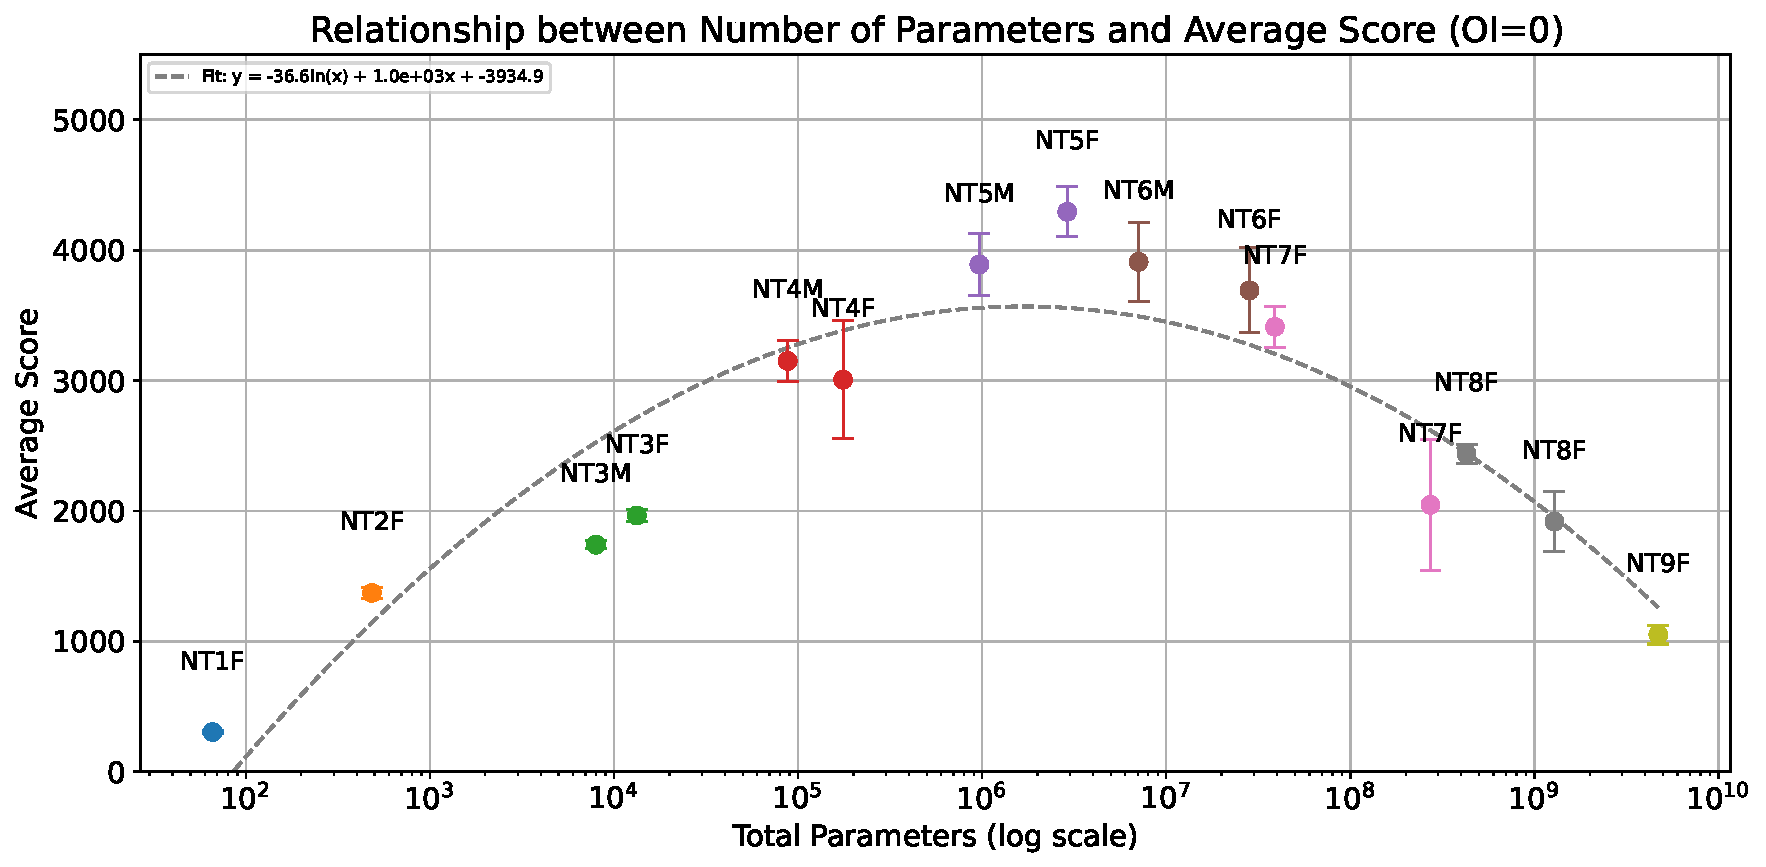
\includegraphics[width=\linewidth]{pdf/parameter_performance_plots/params_performance_OI0_EXP1.pdf}
        \caption{タプル数の変化によるスコアの変化(OI=0)}
        \label{fig:score_vs_tuple_OI0}
    \end{subfigure}

    \vspace{1em}
    \begin{subfigure}[b]{\linewidth}
        \centering
        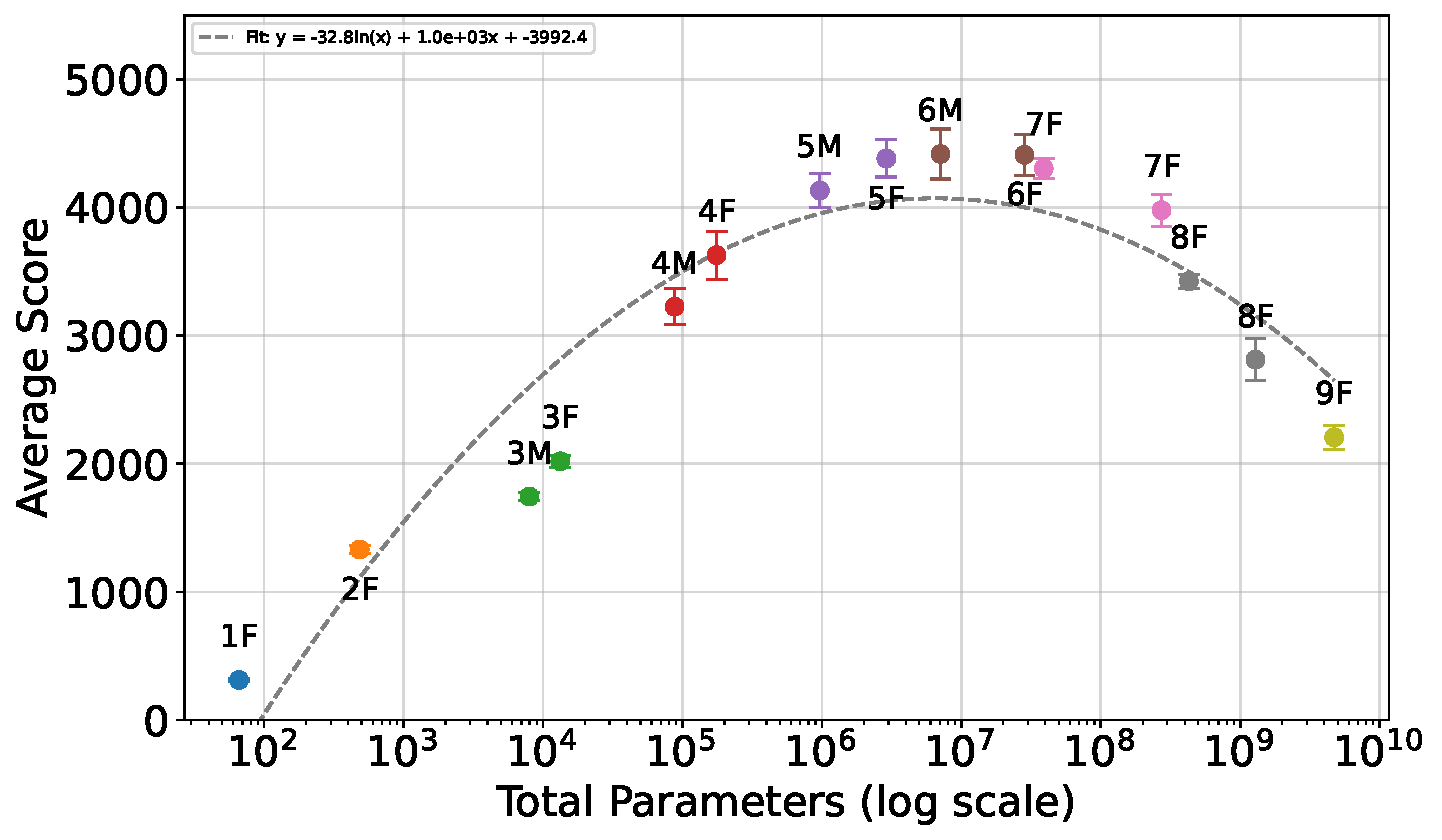
\includegraphics[width=\linewidth]{pdf/parameter_performance_plots/params_performance_OI1200_EXP1.pdf}
        \caption{タプル数の変化によるスコアの変化(OI=1200)}
        \label{fig:score_vs_tuple_OI1200}
    \end{subfigure}

    \vspace{1em}
    \begin{subfigure}[b]{\linewidth}
        \centering
        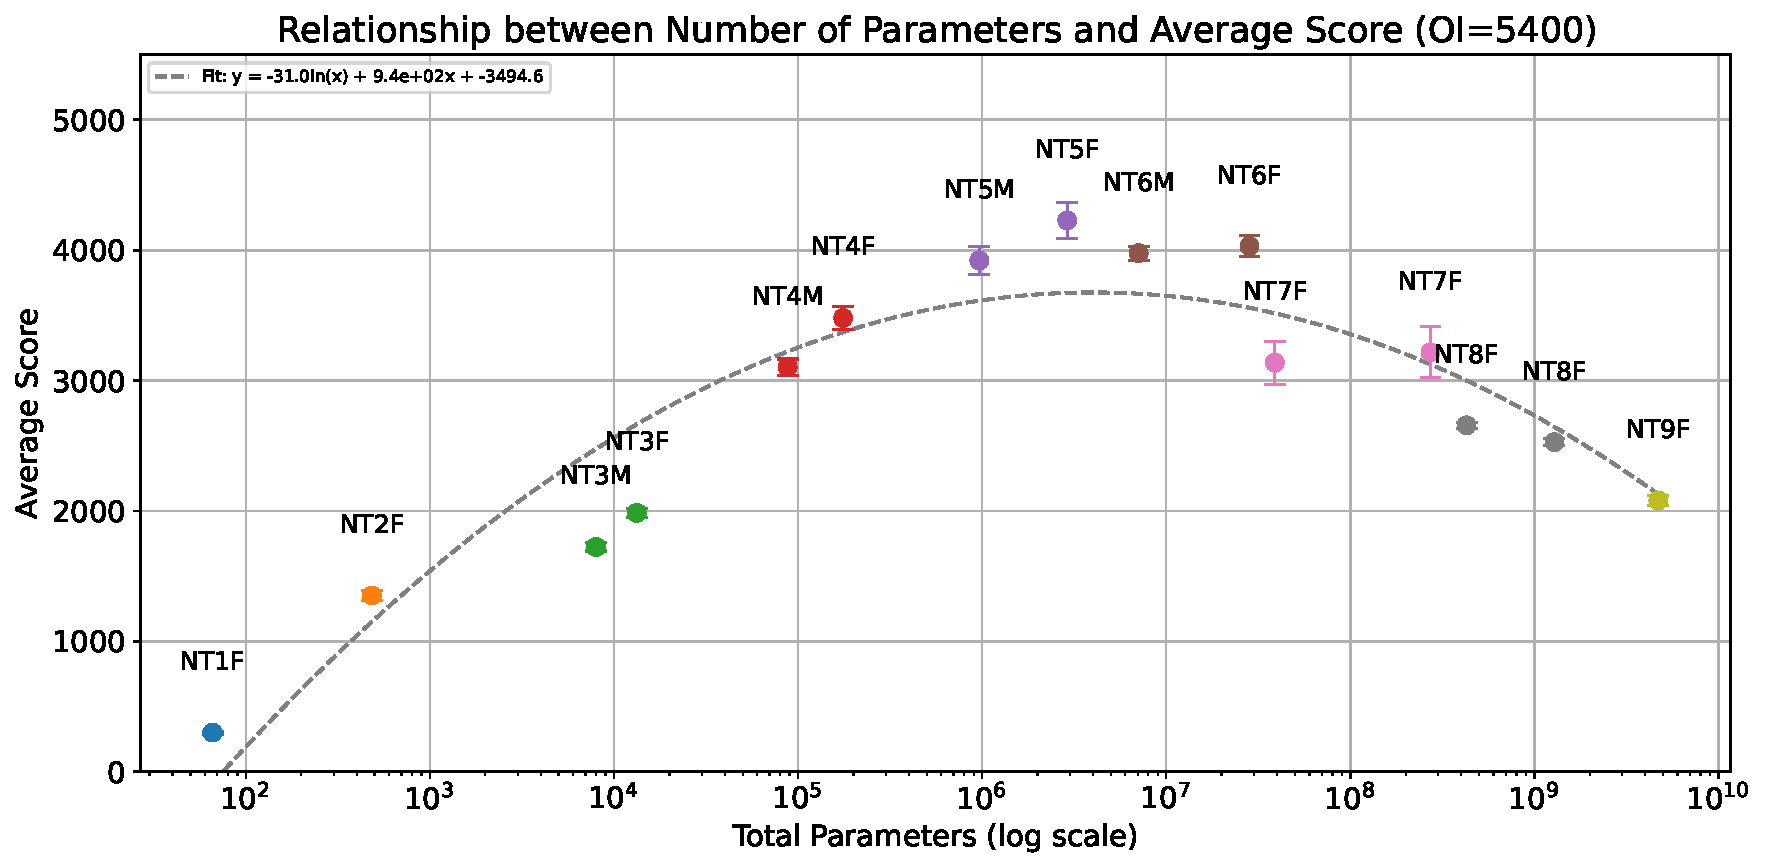
\includegraphics[width=\linewidth]{pdf/parameter_performance_plots/params_performance_OI5400_EXP1.pdf}
        \caption{タプル数の変化によるスコアの変化(OI=5400)}
        \label{fig:score_vs_tuple_OI5400}
    \end{subfigure}

    \caption{OIの初期値ごとのタプル数の変化によるスコアの変化}
    \label{fig:score_vs_tuple_all}
\end{figure}

\begin{figure}[t]
    \centering
    \begin{subfigure}[b]{\linewidth}
        \centering
        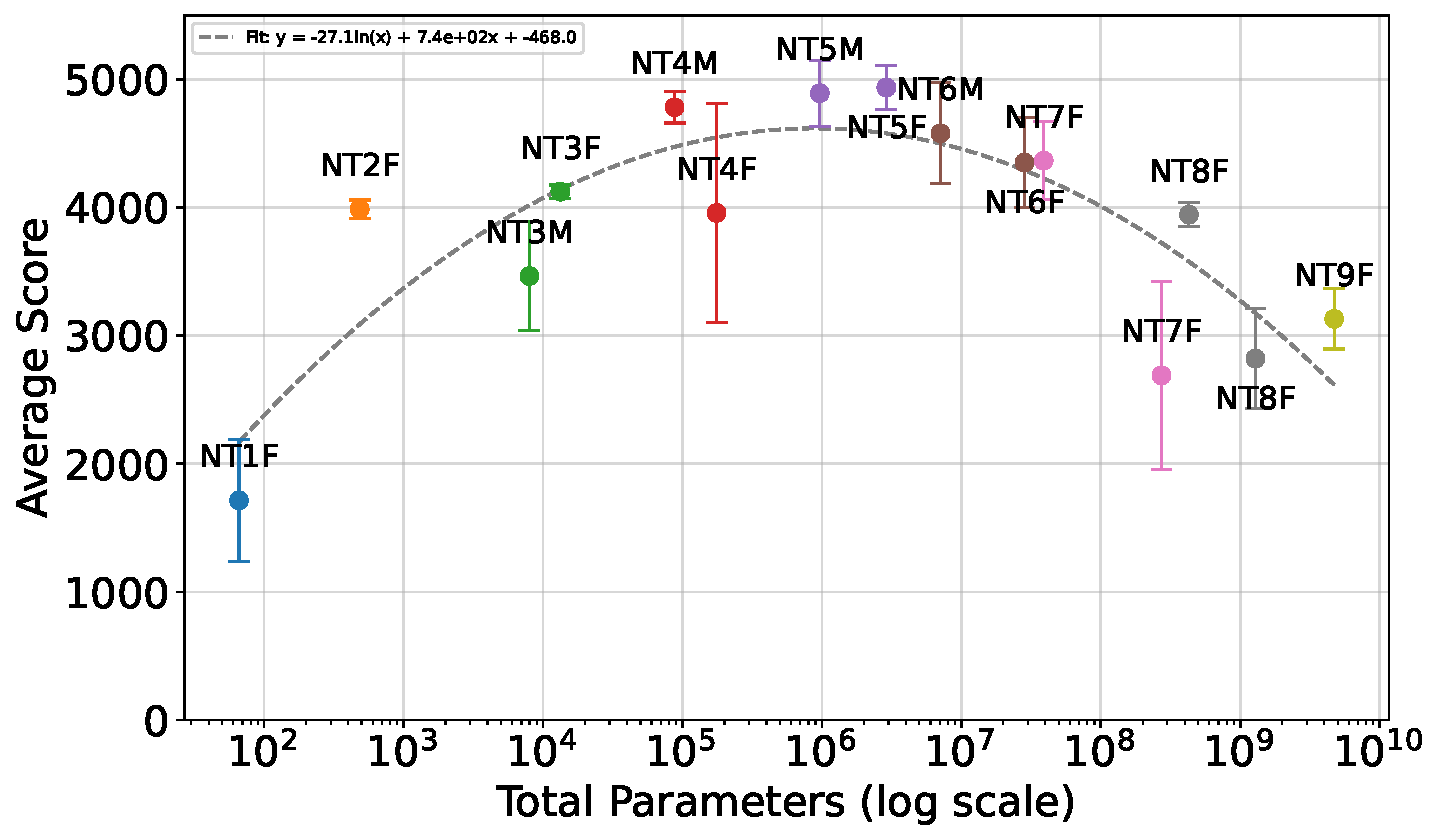
\includegraphics[width=\linewidth]{pdf/parameter_performance_plots/params_performance_OI0_EXP6.pdf}
        \caption{タプル数の変化によるスコアの変化 深さ6(OI=0)}
        \label{fig:score_vs_tuple_OI0_EXP6}
    \end{subfigure}

    \vspace{1em}
    \begin{subfigure}[b]{\linewidth}
        \centering
        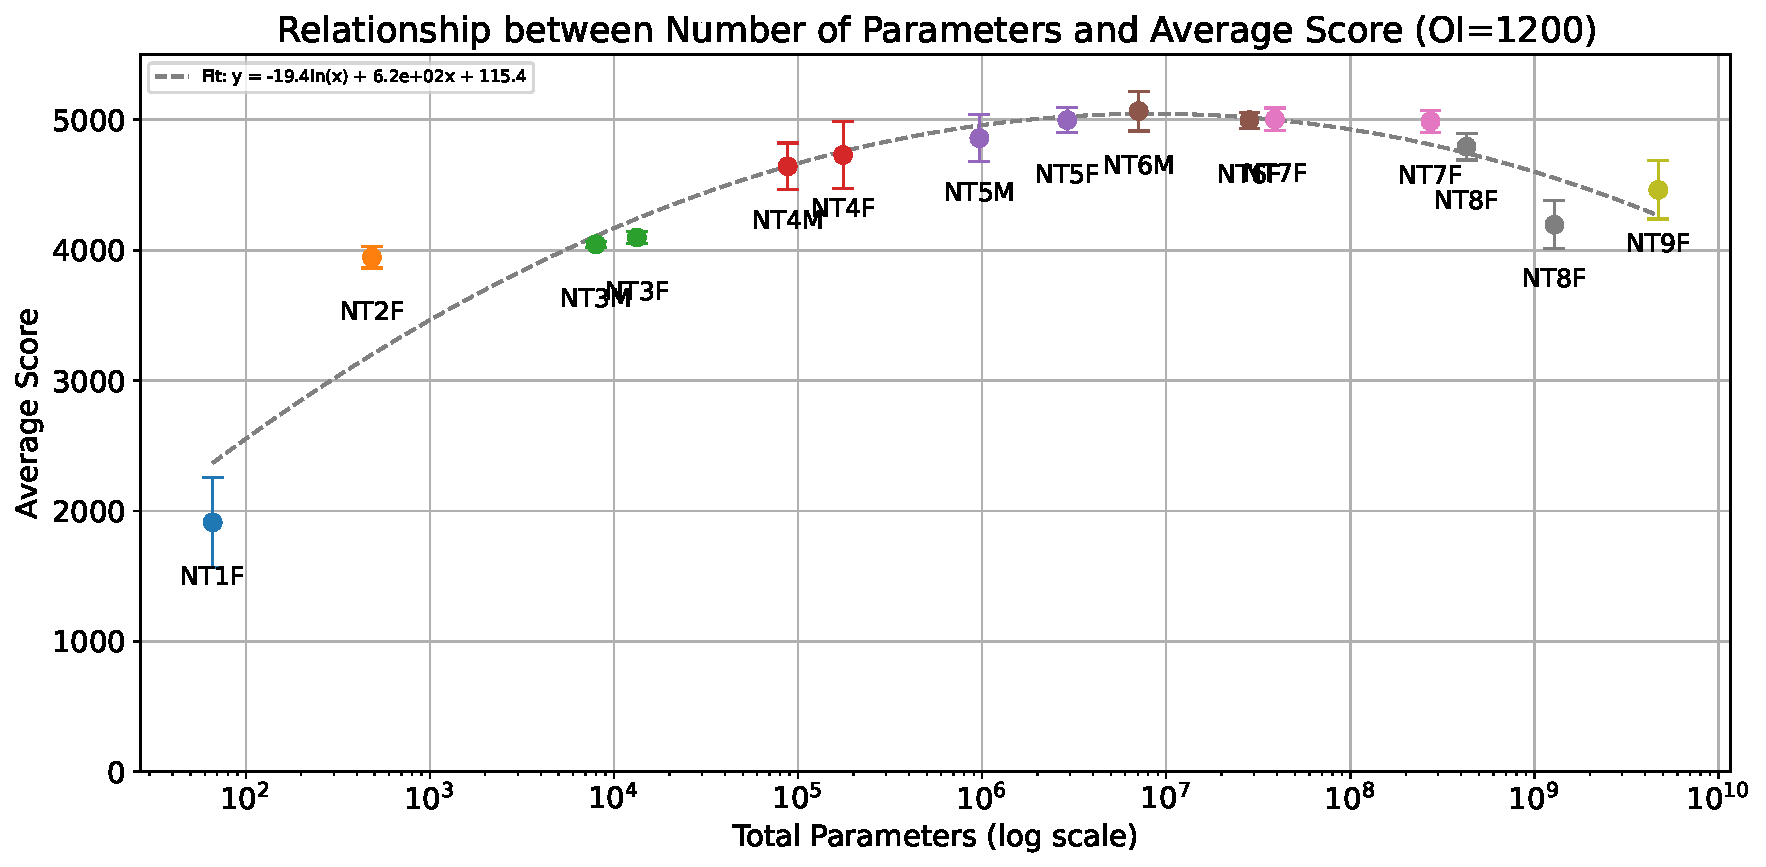
\includegraphics[width=\linewidth]{pdf/parameter_performance_plots/params_performance_OI1200_EXP6.pdf}
        \caption{タプル数の変化によるスコアの変化 深さ6(OI=1200)}
        \label{fig:score_vs_tuple_OI1200_EXP6}
    \end{subfigure}

    \vspace{1em}
    \begin{subfigure}[b]{\linewidth}
        \centering
        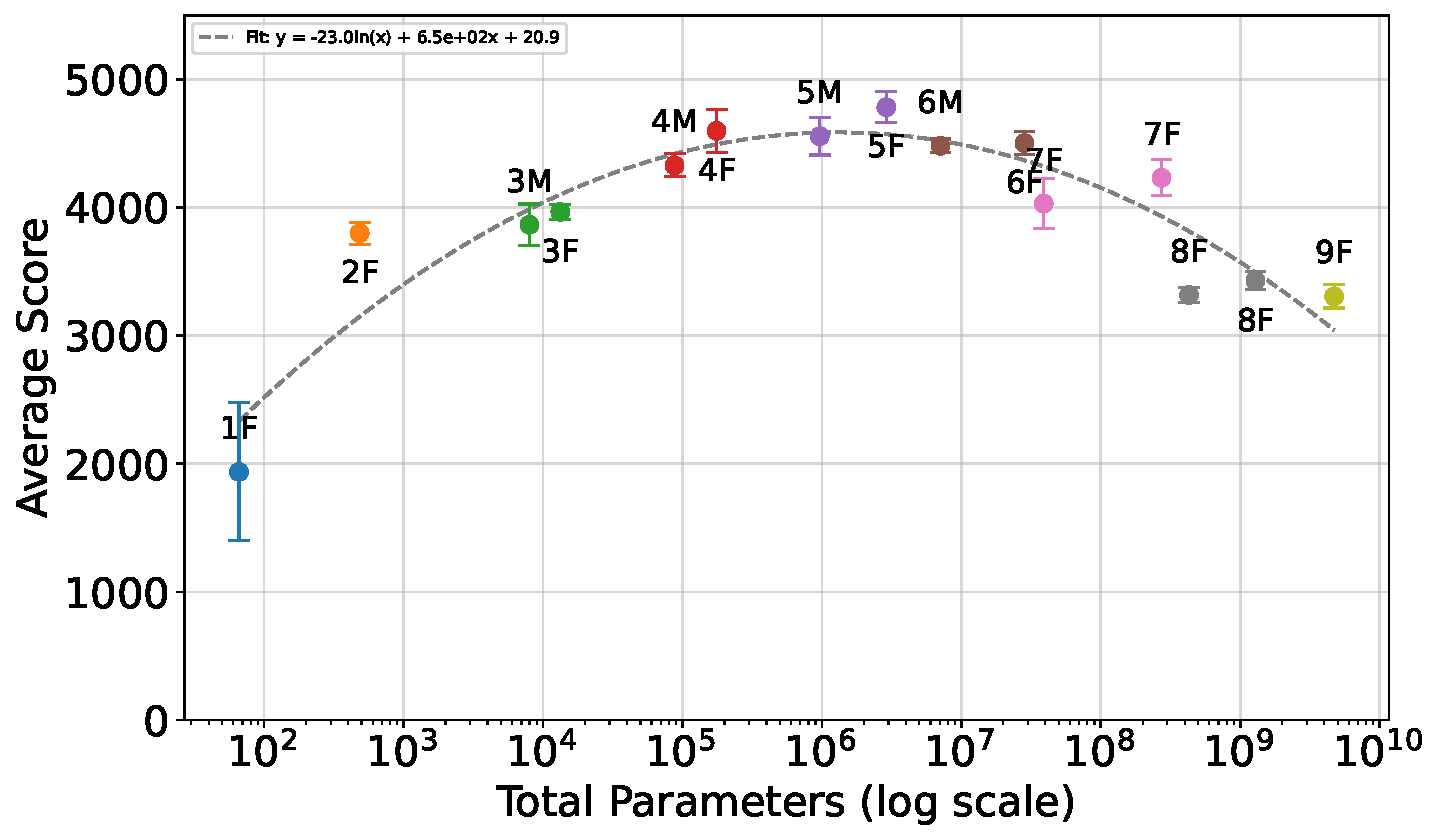
\includegraphics[width=\linewidth]{pdf/parameter_performance_plots/params_performance_OI5400_EXP6.pdf}
        \caption{タプル数の変化によるスコアの変化 深さ6(OI=5400)}
        \label{fig:score_vs_tuple_OI5400_EXP6}
    \end{subfigure}

    \caption{Expectimax深さ6でのOIの初期値ごとのタプル数の変化によるスコアの変化}
    \label{fig:score_vs_tuple_all_EXP6}
\end{figure}

図\ref{fig:score_vs_tuple_OI0_EXP6}から図\ref{fig:score_vs_tuple_OI5400_EXP6}は、OIの初期値を変えた場合の各プレイヤとExpectimaxの深さ6を組み合わせたプレイヤでの、
パラメータ数の対数とスコアの関係を示している。
いずれのグラフも放物線を描いていること、いずれの平均の平均のスコアもGreedyプレイのスコアよりも高いことが確認できた。
また、OIの初期値を0に設定した場合、探索を加えてもスコアのバラつきが多いプレイヤが見られた、特にFullタプルのスコアのバラつきが大きいことが確認できた。
これはパラメータ数が多い方が評価値の修正が起こり難く、局所最適解から抜け出しにくいのではないかと考えられる。
またOIの初期値を1200に設定したばあいNT5MからNT7Fまでスコアにほとんど差がなく、放物線の上昇と下降の傾きが小さくなっていることが確認できた。
これは強いプレイヤはNタプルプレイヤの現実的なスコア上限に近づいていて、ほとんど上昇しないことと、
弱いプレイヤは探索によってスコアが上昇することを示している。
またOIの初期値を5400に設定した場合、平均の標準偏差はとても小さくなったが、放物線の形やスコアの上限はOIの初期値0の時とあまり変わらなかった。

\begin{figure}[t]
    \centering
    % OI=0の比較
    \begin{subfigure}[b]{0.49\linewidth}
        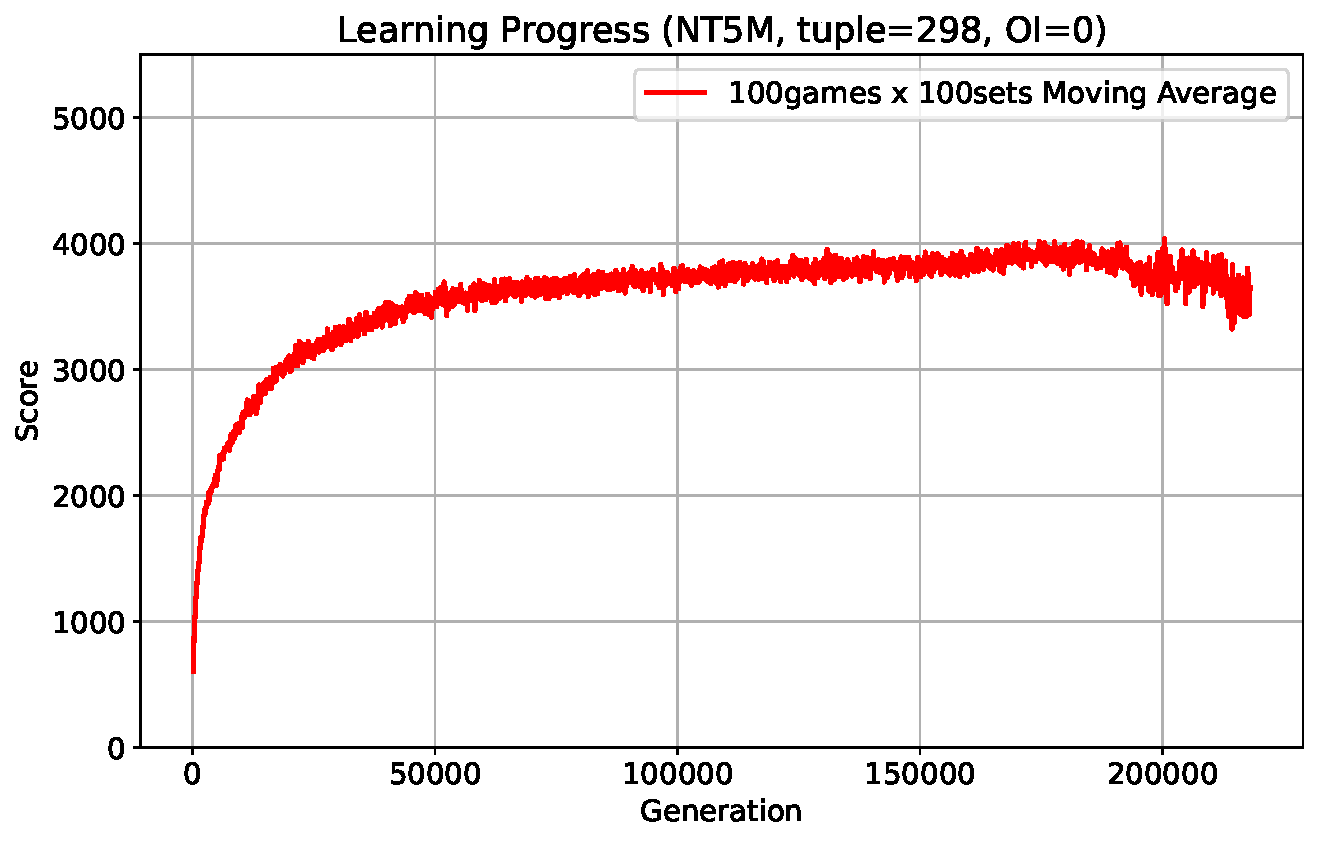
\includegraphics[width=\linewidth]{pdf/learning_progress_plots/learning_progress_NT5_tuple298_OI0.pdf}
        \caption{NT5M,OI=0学習推移}
        \label{fig:NT5F_OI0_learning_progress}
    \end{subfigure}
    \begin{subfigure}[b]{0.49\linewidth}
        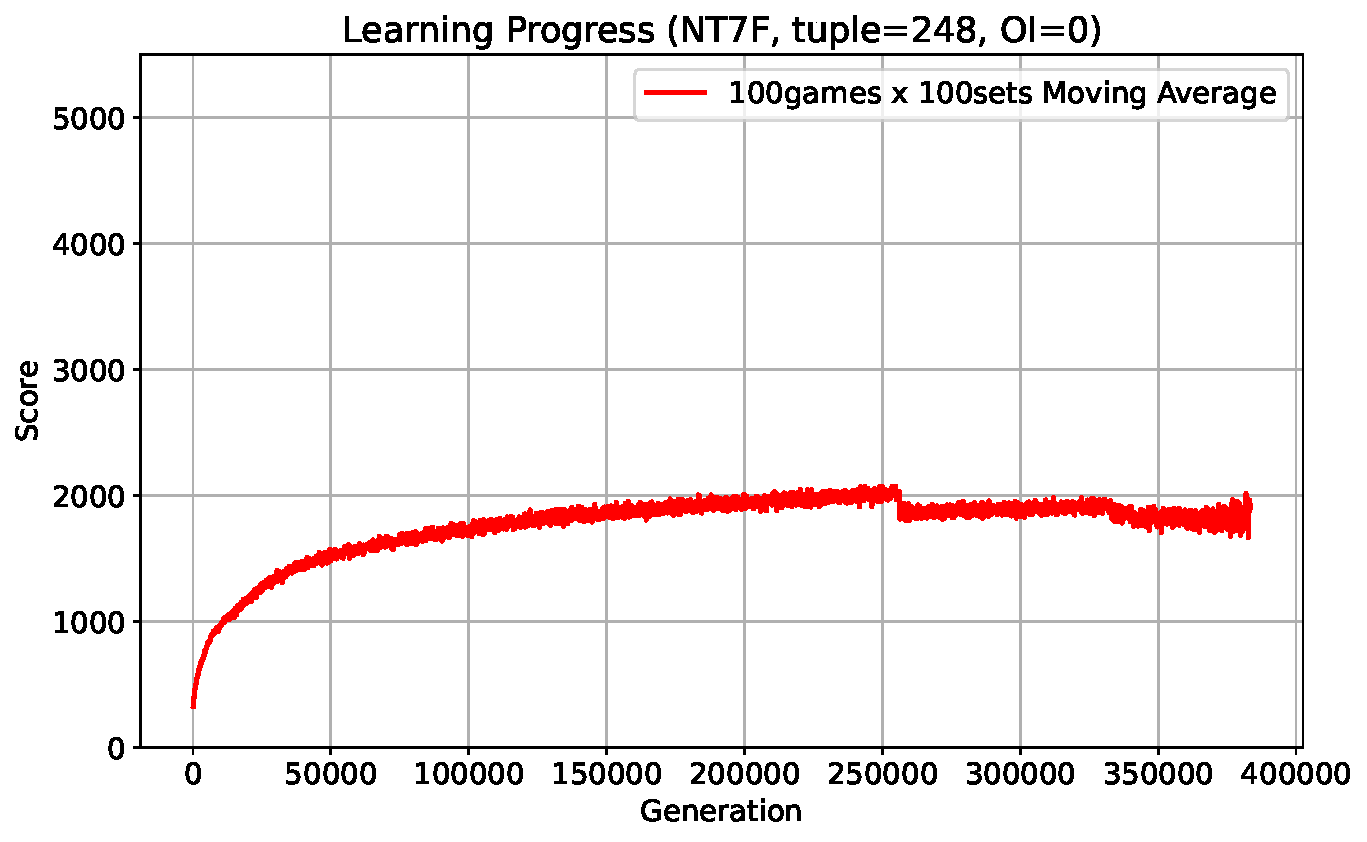
\includegraphics[width=\linewidth]{pdf/learning_progress_plots/learning_progress_NT7_tuple248_OI0.pdf}
        \caption{NT7F,OI=0学習推移}
        \label{fig:NT7F_OI0_learning_progress}
    \end{subfigure}

    \vspace{1em}
    % OI=1200の比較
    \begin{subfigure}[b]{0.49\linewidth}
        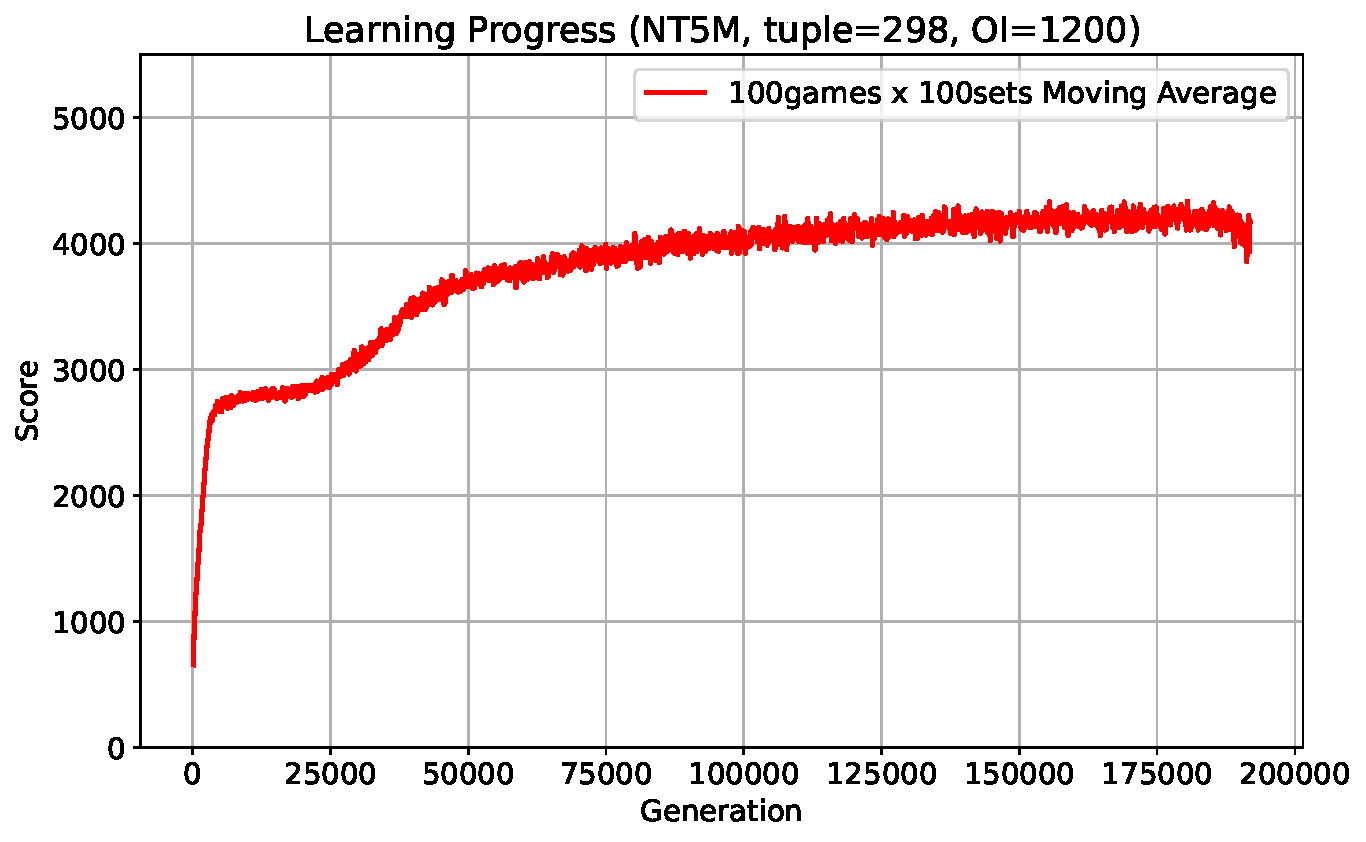
\includegraphics[width=\linewidth]{pdf/learning_progress_plots/learning_progress_NT5_tuple298_OI1200.pdf}
        \caption{NT5M,OI=1200学習推移}
        \label{fig:NT5M_OI1200_learning_progress}
    \end{subfigure}
    \begin{subfigure}[b]{0.49\linewidth}
        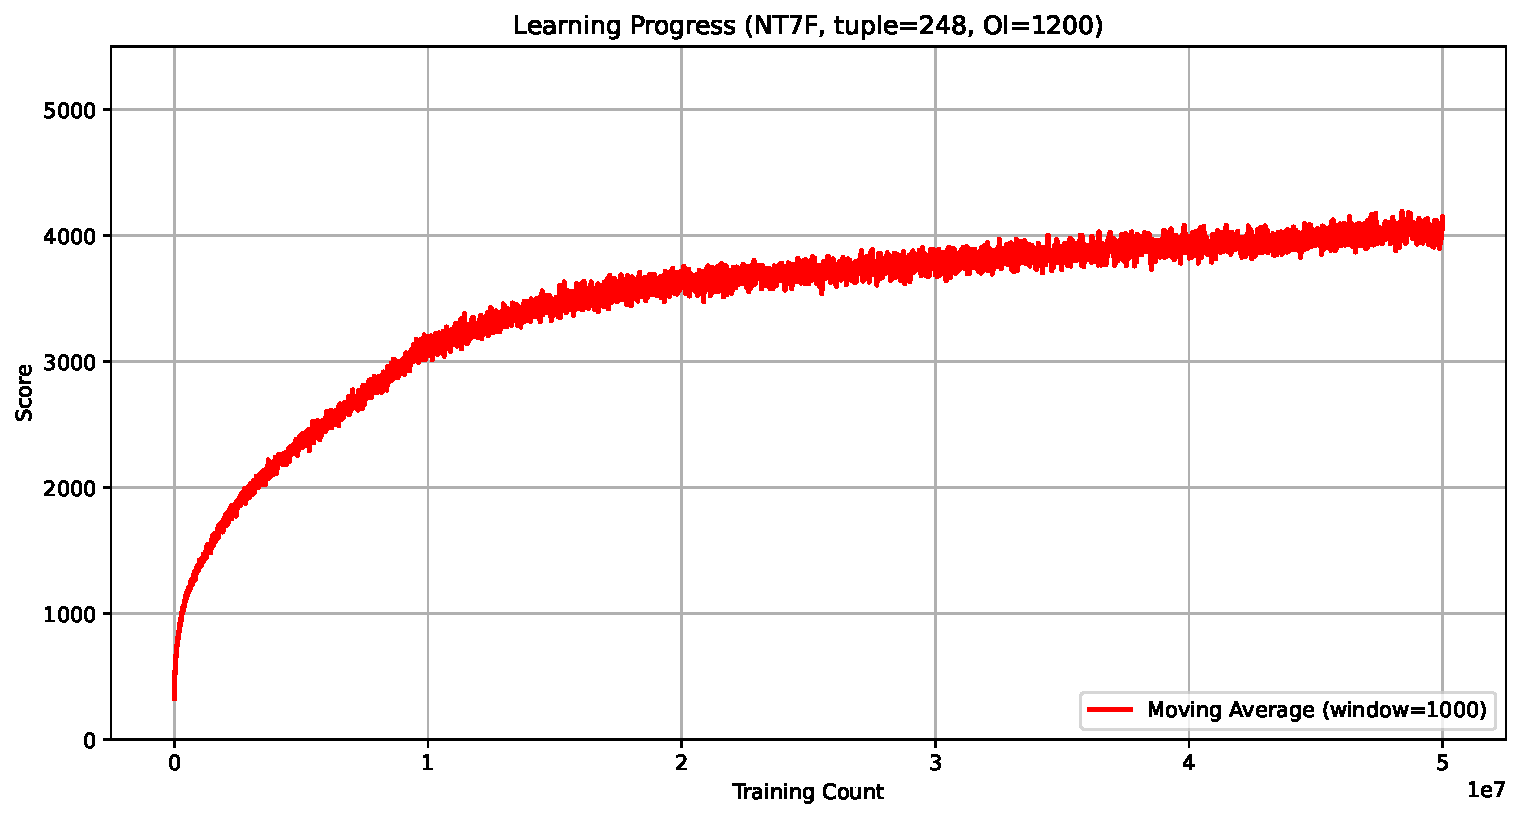
\includegraphics[width=\linewidth]{pdf/learning_progress_plots/learning_progress_NT7_tuple248_OI1200.pdf}
        \caption{NT7F,OI=1200学習推移}
        \label{fig:NT7F_OI1200_learning_progress}
    \end{subfigure}

    \vspace{1em}
    % OI=5400の比較
    \begin{subfigure}[b]{0.49\linewidth}
        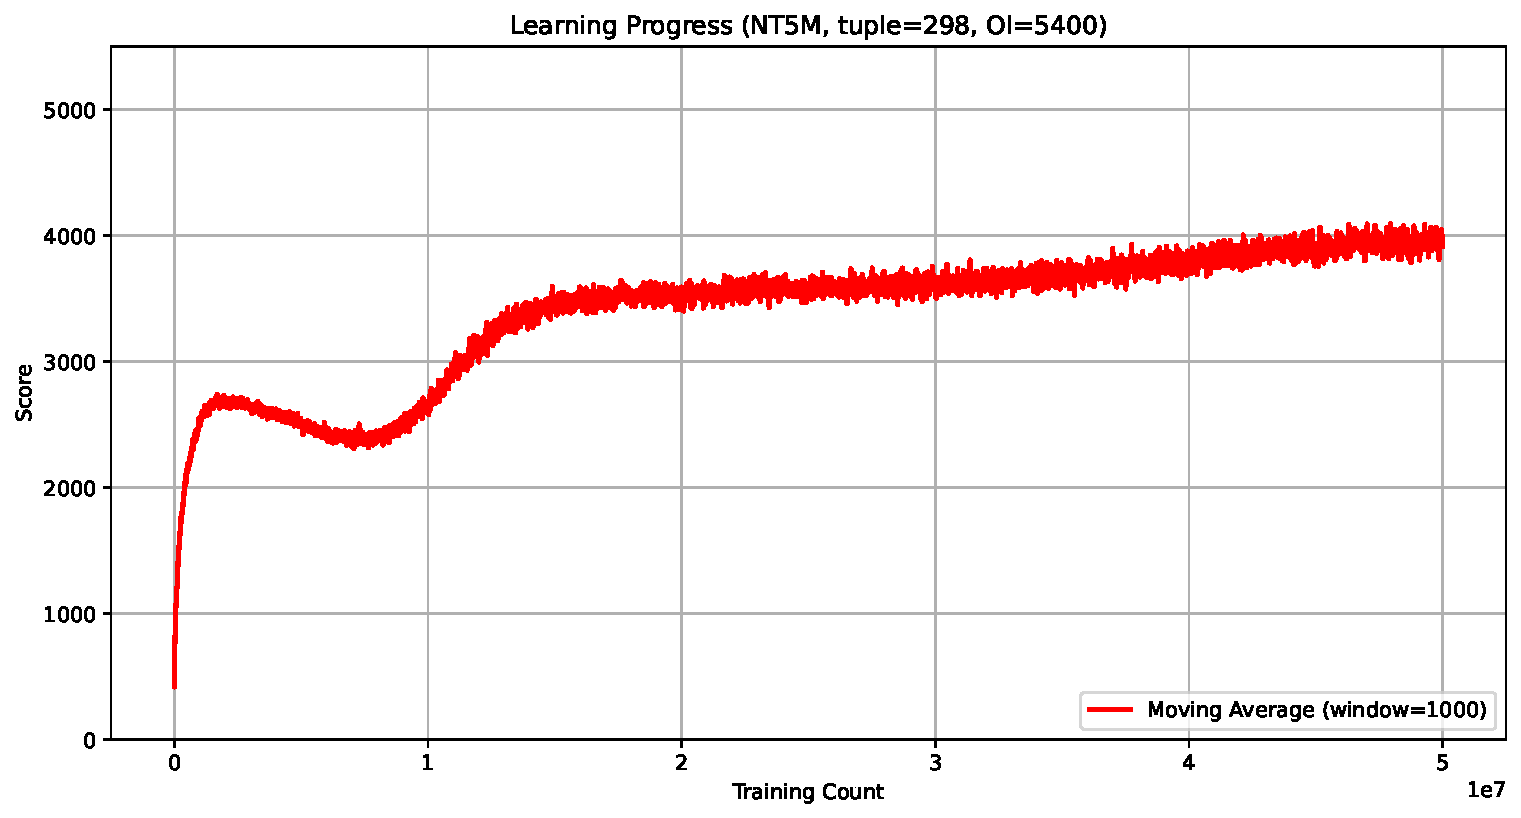
\includegraphics[width=\linewidth]{pdf/learning_progress_plots/learning_progress_NT5_tuple298_OI5400.pdf}
        \caption{NT5M,OI=5400学習推移}
        \label{fig:NT5M_OI5400_learning_progress}
    \end{subfigure}
    \begin{subfigure}[b]{0.49\linewidth}
        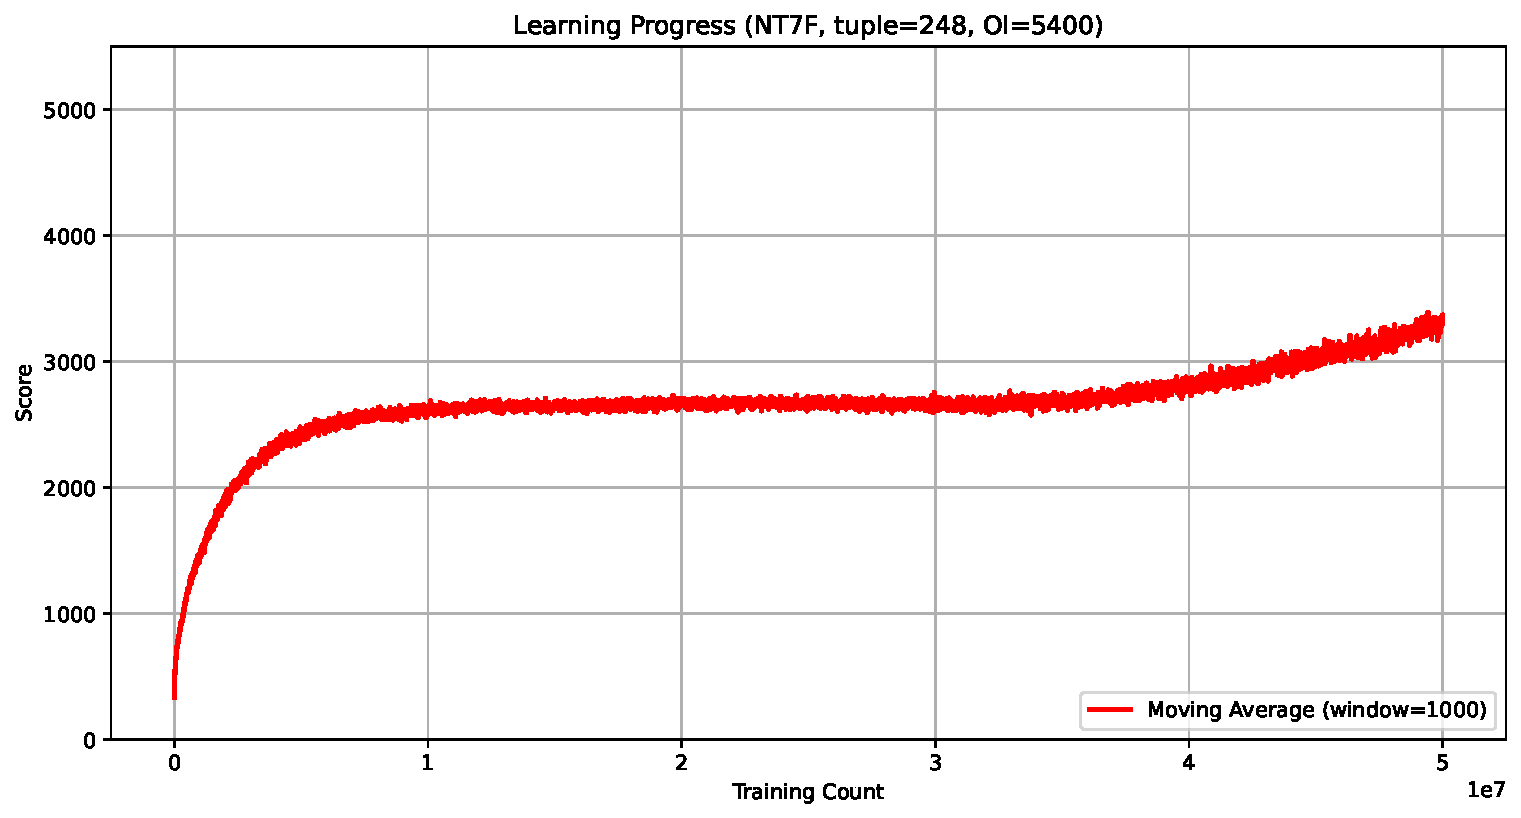
\includegraphics[width=\linewidth]{pdf/learning_progress_plots/learning_progress_NT7_tuple248_OI5400.pdf}
        \caption{NT7F,OI=5400学習推移}
        \label{fig:NT7F_OI5400_learning_progress}
    \end{subfigure}

    \caption{NT5MとNT7Fの学習推移の比較}
    \label{fig:learning_progress_comparison}
\end{figure}

図\ref{fig:learning_progress_comparison}は、NT5MとNT7Fの学習の際のスコアの推移を示している。
このグラフではy軸にスコア,x軸に学習回数を取り、各学習回数ごとのスコアの平均を求め、
それを学習回数10000ごとに移動平均を取り、グラフにプロットしている。

OIの初期値を0に設定した場合(図\ref{fig:NT5M_OI0_learning_progress},図\ref{fig:NT7F_OI0_learning_progress})、NT5Mは学習が進むにつれてスコアが上昇しているが、NT7Fはスコアが上昇しないことが確認できた。
これはNT7Fが局所最適解にハマっていることを示している。
OIの初期値を1200に設定した場合(図\ref{fig:NT5M_OI1200_learning_progress},図\ref{fig:NT7F_OI1200_learning_progress})、NT5MとNT7Fの両方のスコアの上昇が緩やかになり、
NT5Mの場合学習途中スコアとしては約2800点ほどで一度停滞が入り、その後再び上昇に転じている。
このスコアの停滞しているのは表\ref{specific}を見ると256タイルが完成してから512タイルが完成するまでの間であることが分かる。
この停滞期の盤面は盤面に比較的空きタイルがあり、色んな手を選択することで効率の悪い手を選んでしまい停滞しているのではないかと考えている。
また、NT7FはOIの初期値を1200に設定した場合、序盤のスコアの上昇が緩やかになっているのも同じ原因ではないかと考える。
OIの初期値を5400に設定した場合(図\ref{fig:NT5M_OI5400_learning_progress},図\ref{fig:NT7F_OI5400_learning_progress})、NT5MとNT7Fの両方のスコアの上昇が緩やかになり、、両方とも途中で停滞が発生している。
NT5Mは停滞を乗り越えて大きくスコアを上昇させているが、NT7Fは停滞が長引き大きなスコア上昇にまで至っていないので、
学習不足であると考えている。

\subsection{パラメータ数の増加によるプレイヤの挙動の変化}
ここからOIの初期値1200のスコアが同等でパラメータ数が違うNT4FとNT8M、NT5MとNT7Fのプレイヤを比較して、
パラメータ数の増加がプレイヤの挙動にどのような影響を与えるのかについて詳しく調べて行く。
\begin{figure}[t]
\centering
\begin{subfigure}[b]{0.49\linewidth}
    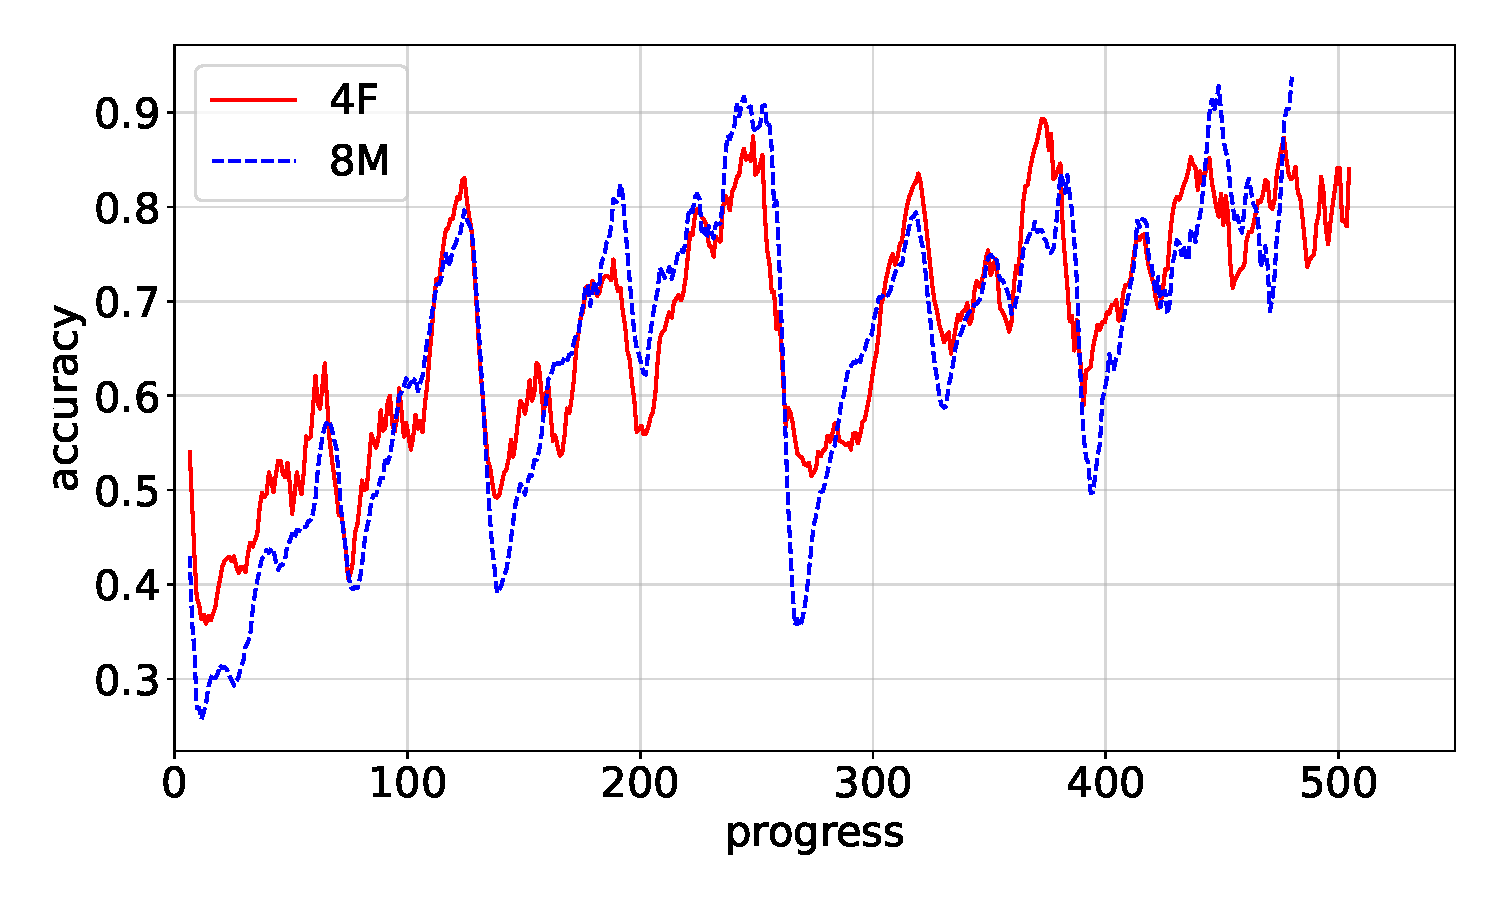
\includegraphics[width=\linewidth]{pdf/compare/NT4F_and_NT8M/accuracy.pdf}
    \caption{正確度}
    \label{fig:NT4F_and_NT8M_accuracy}
\end{subfigure}
\begin{subfigure}[b]{0.49\linewidth}
    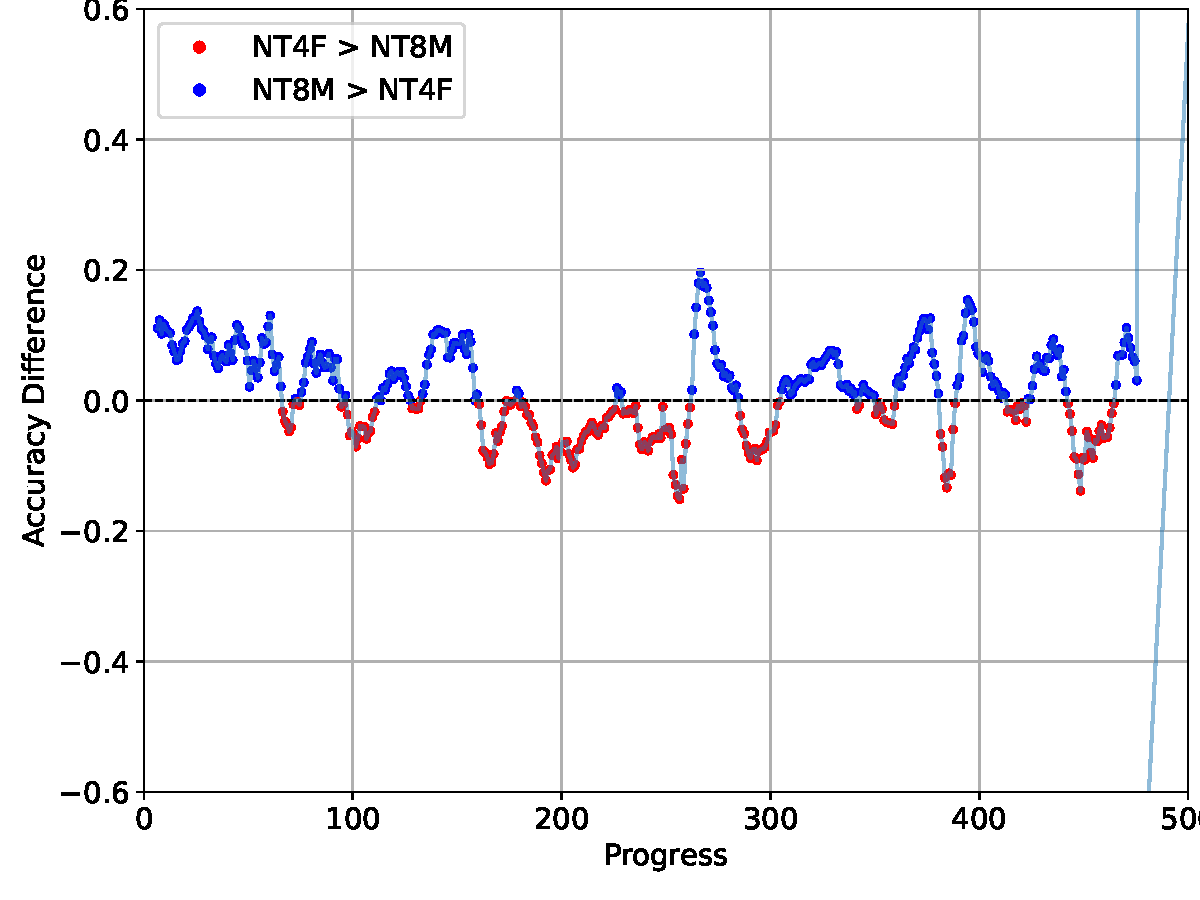
\includegraphics[width=\linewidth]{pdf/compare/NT4F_and_NT8M/acc_diff_plot.pdf}
    \caption{正確度の差分}
    \label{fig:NT4F_and_NT8M_acc_diff}
\end{subfigure}
\begin{subfigure}[b]{0.49\linewidth}
    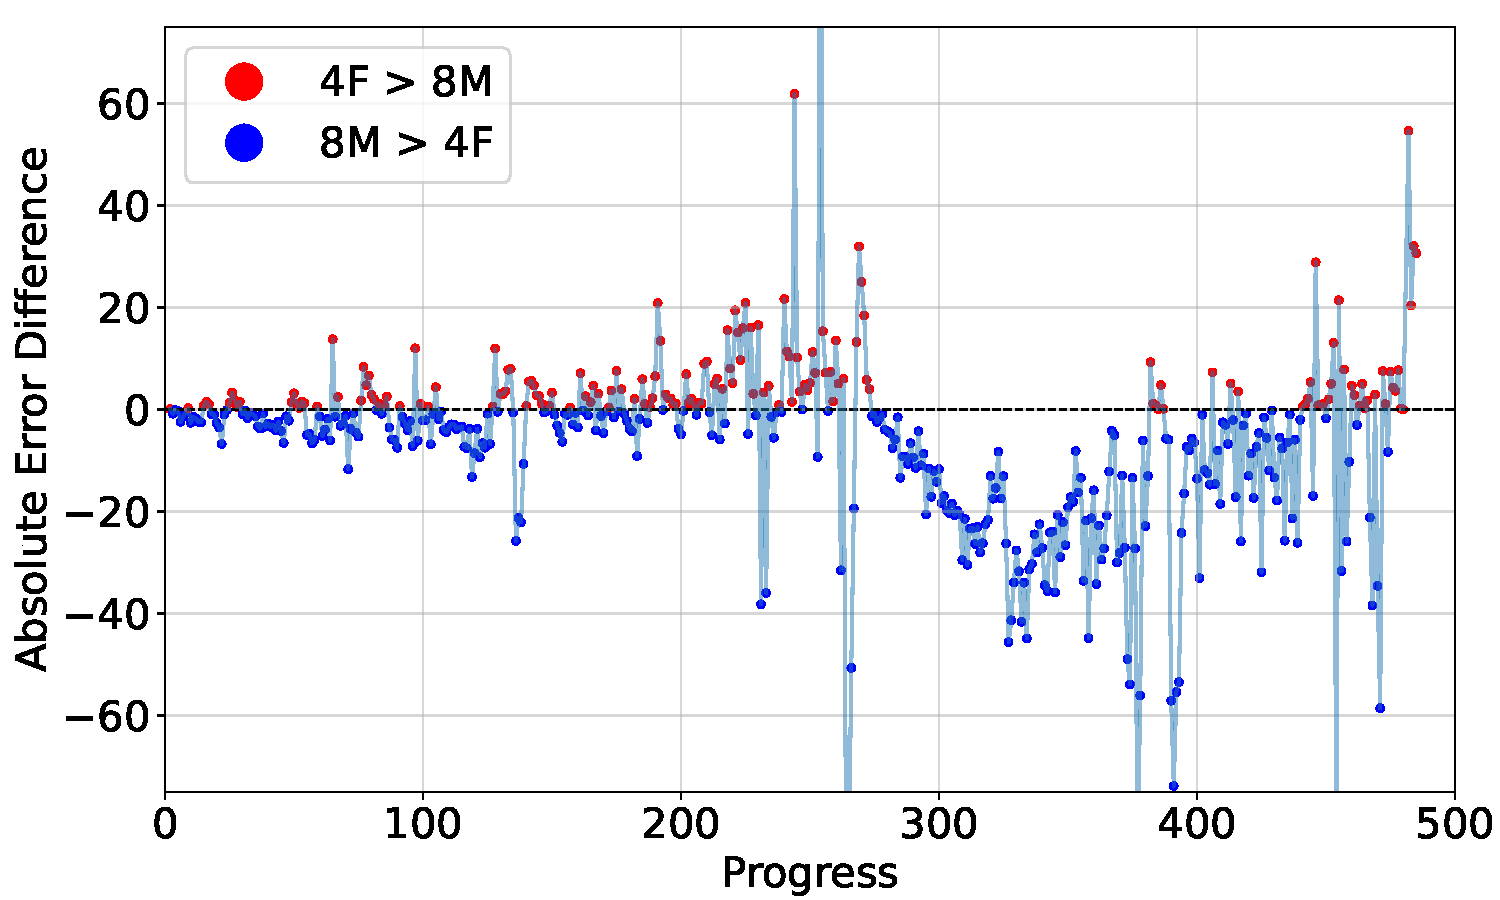
\includegraphics[width=\linewidth]{pdf/compare/NT4F_and_NT8M/error_abs_diff_plot.pdf}
    \caption{絶対誤差の差分}
    \label{fig:NT4F_and_NT8M_error_abs_diff}
\end{subfigure}
\begin{subfigure}[b]{0.49\linewidth}
    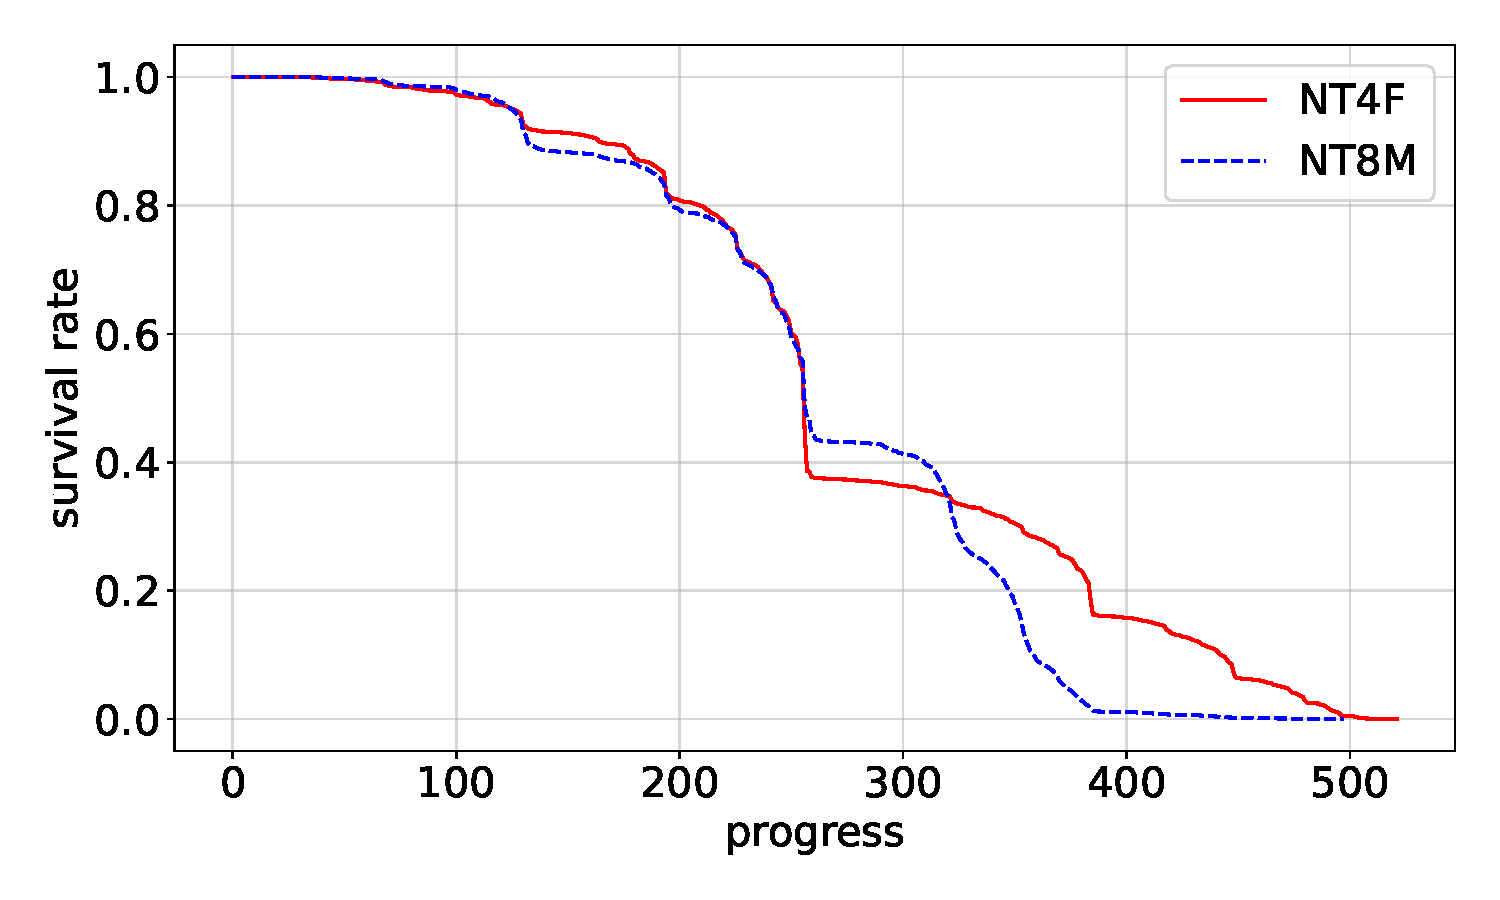
\includegraphics[width=\linewidth]{pdf/compare/NT4F_and_NT8M/survival.pdf}
    \caption{生存率}
    \label{fig:NT4F_and_NT8M_survival}
\end{subfigure}
\caption{NT4FとNT8Mの比較結果}
\label{fig:NT4FとNT8M_results}
\end{figure}

まず初めに図\ref{fig:NT4F_and_NT8M_results}は、NT4FとNT8MのプレイヤのGreedyプレイの比較を示している。
\ref{fig:NT4F_and_NT8M_accuracy}と\ref{fig:NT4F_and_NT8M_acc_diff}は、NT4FとNT8Mのプレイヤの正確度を示している。
これを見ると序盤はNT4Fの方が正確度が高いが、中盤以降はどちらも抜きつ抜かれつの状態であることが分かる。
\ref{fig:NT4F_and_NT8M_error_abs_diff}は、NT4FとNT8Mのプレイヤの絶対誤差の差分を示している。
これを見ると、NT4Fの方がNT8M多くのprogressで絶対誤差が小さいことが分かる。
正確度のグラフと絶対誤差のグラフを合わせてみると、NT4Fの方が後半かなり良いことがわかる。
これは\ref{fig:NT4F_and_NT8M_survival}の生存率のグラフにも表れている。

\begin{figure}[t]
\centering
\begin{subfigure}[b]{0.49\linewidth}
    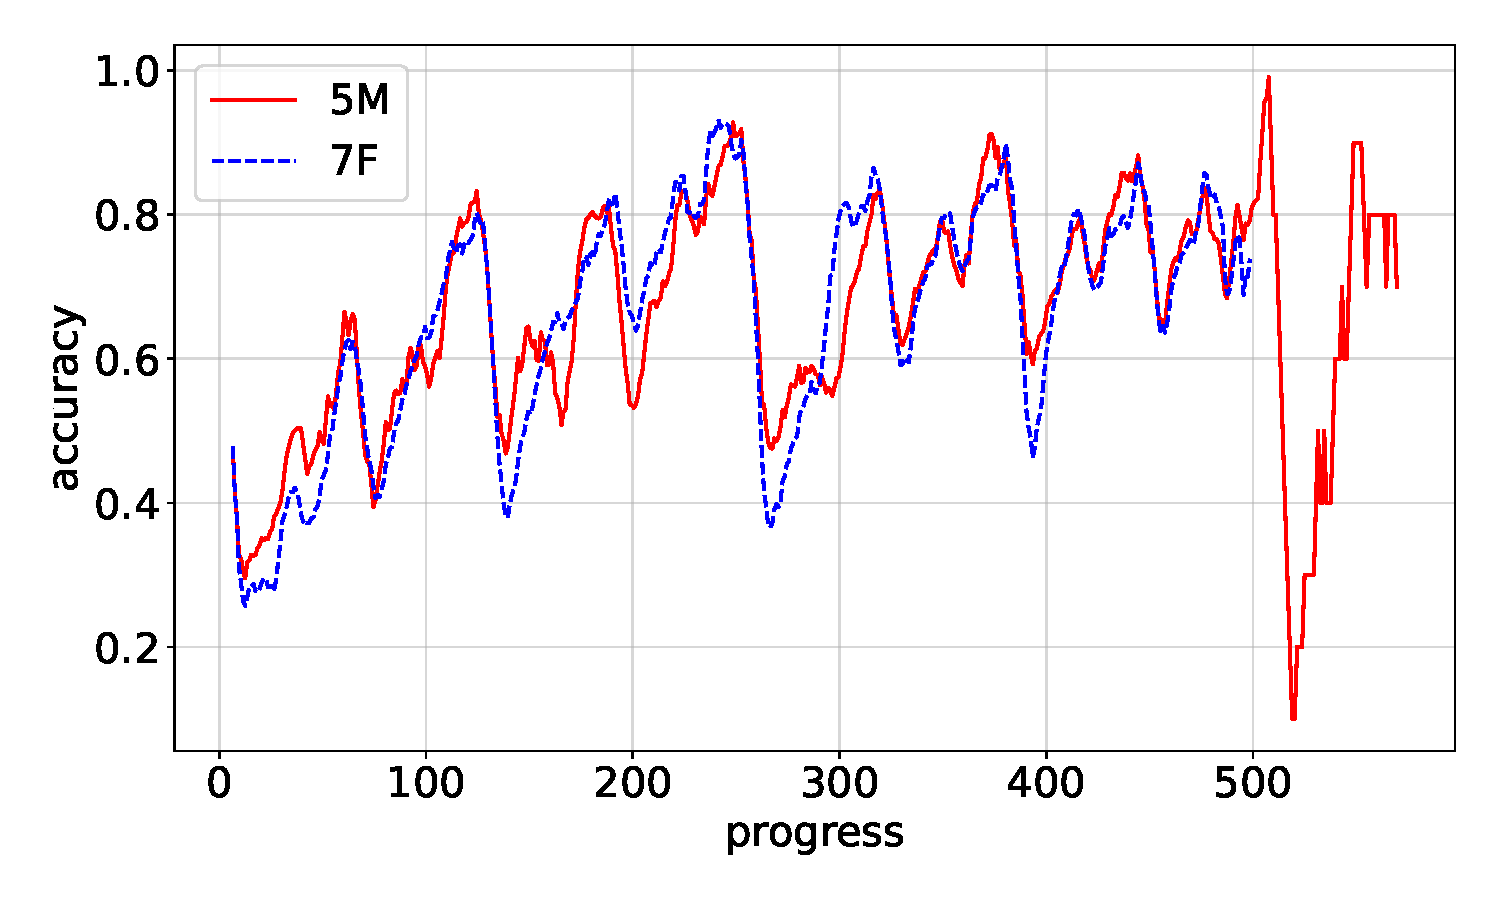
\includegraphics[width=\linewidth]{pdf/compare/NT5M_and_NT7F/accuracy.pdf}
    \caption{正確度}
    \label{fig:NT5M_and_NT7F_accuracy}
\end{subfigure}
\begin{subfigure}[b]{0.49\linewidth}
    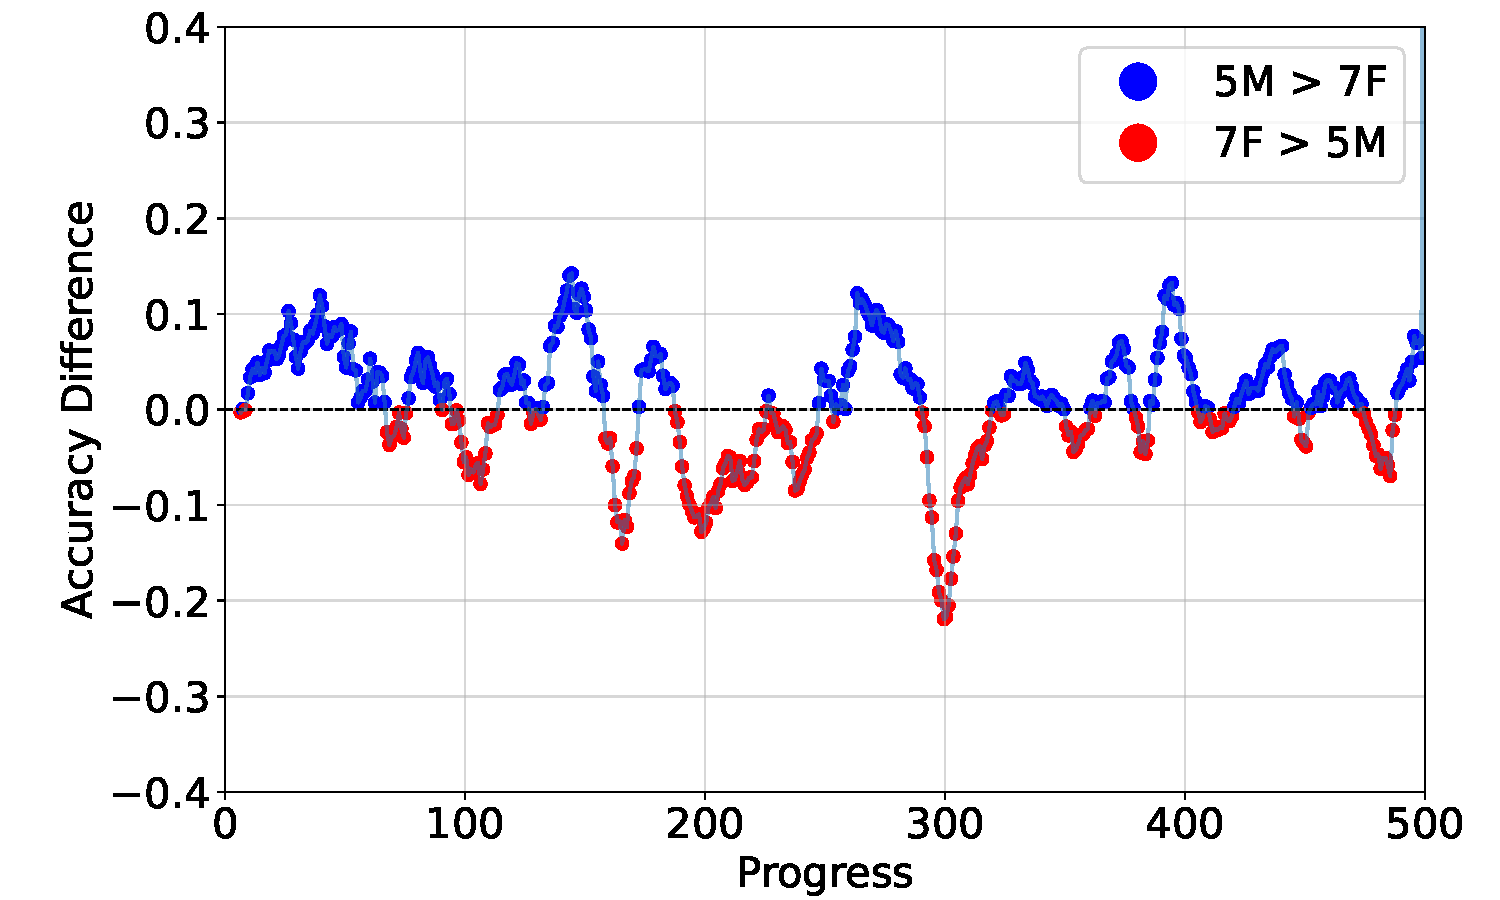
\includegraphics[width=\linewidth]{pdf/compare/NT5M_and_NT7F/acc_diff_plot.pdf}
    \caption{正確度の差分}
    \label{fig:NT5M_and_NT7F_acc_diff}
\end{subfigure}
\begin{subfigure}[b]{0.49\linewidth}
    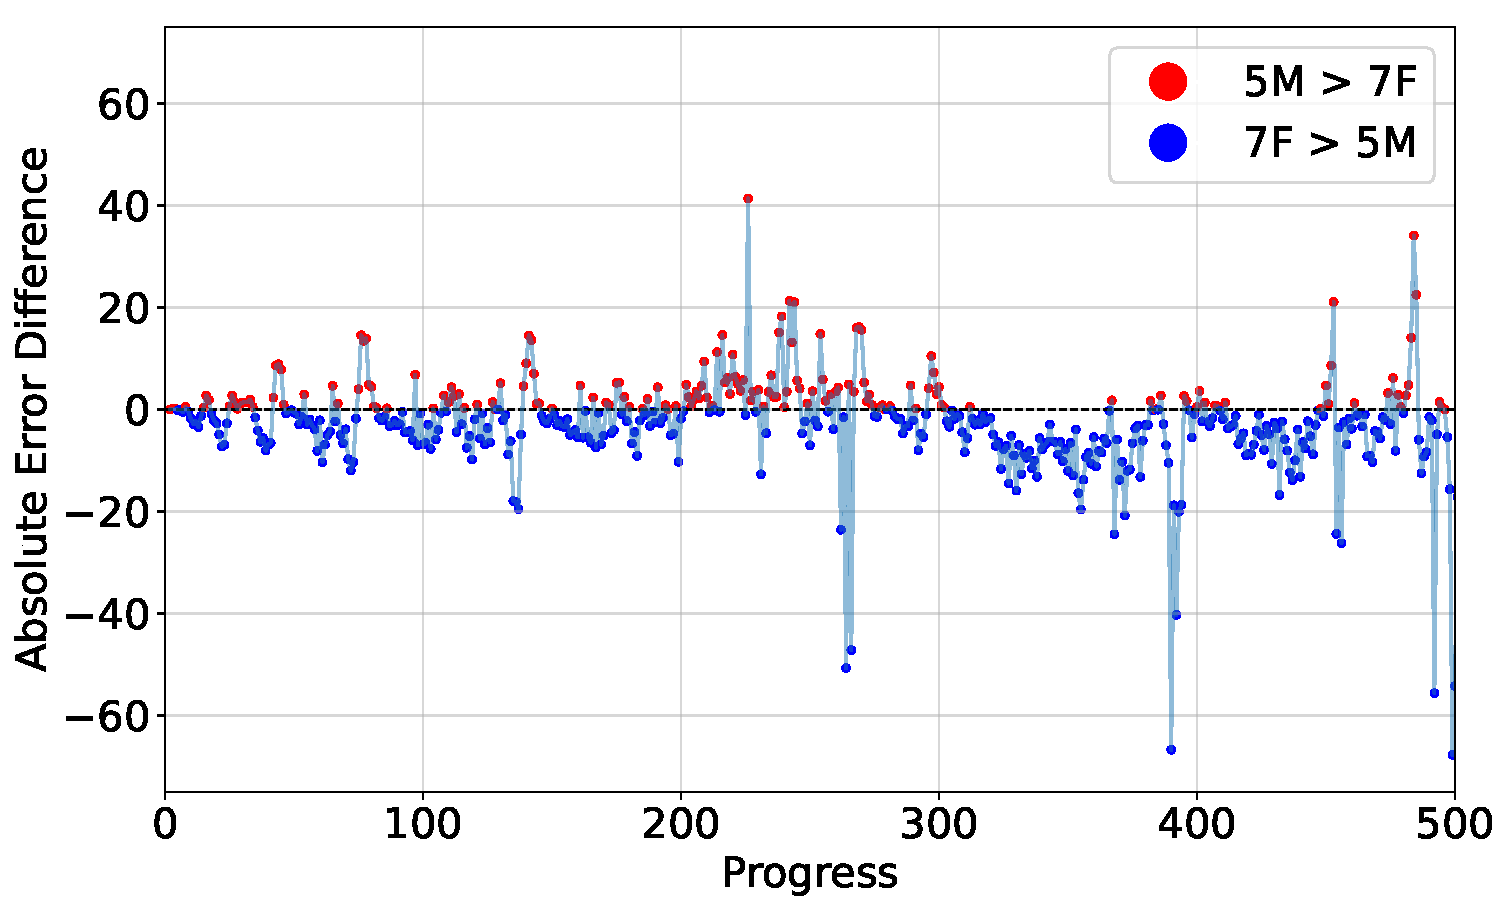
\includegraphics[width=\linewidth]{pdf/compare/NT5M_and_NT7F/error_abs_diff_plot.pdf}
    \caption{絶対誤差の差分}
    \label{fig:NT5M_and_NT7F_error_abs_diff}
\end{subfigure}
\begin{subfigure}[b]{0.49\linewidth}
    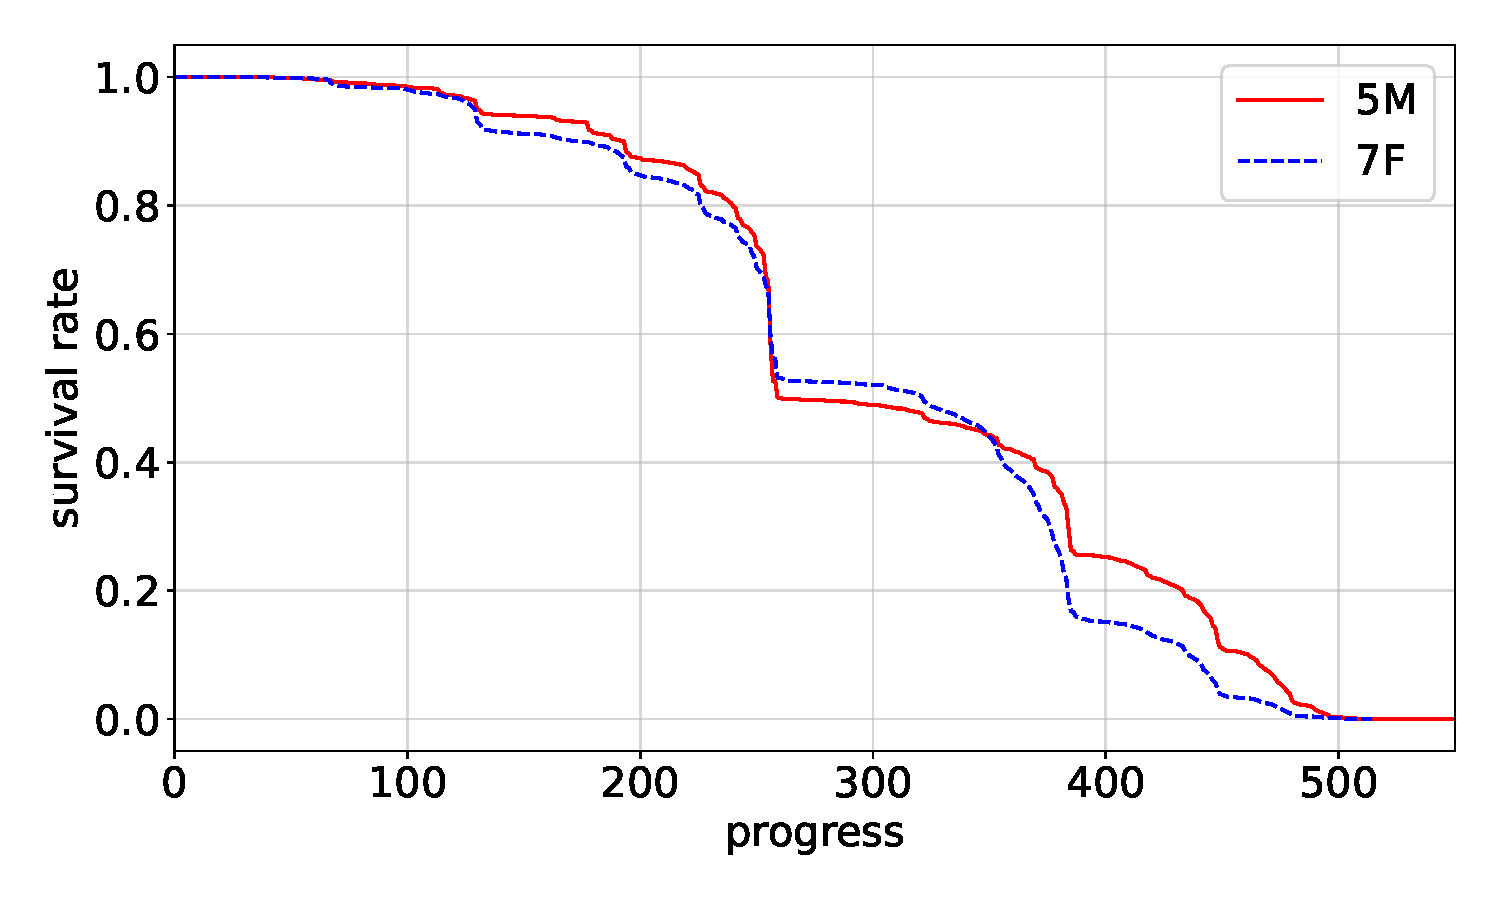
\includegraphics[width=\linewidth]{pdf/compare/NT5M_and_NT7F/survival.pdf}
    \caption{生存率}
    \label{fig:NT5M_and_NT7F_survival}
\end{subfigure}
\caption{NT5MとNT7Fの比較結果}
\label{fig:NT5M_and_NT7F_results}
\end{figure}

次に図\ref{fig:NT5M_and_NT7F_results}は、NT5MとNT7FのプレイヤのGreedyプレイの比較を示している。
\ref{fig:NT5M_and_NT7F_accuracy}と\ref{fig:NT5M_and_NT7F_acc_diff}を見ると
NT5Mの方がNT7Fよりも正確度が高いことが分かる。
\ref{fig:NT5M_and_NT7F_error_abs_diff}は、NT5MとNT7Fのプレイヤの絶対誤差の差分を示している。
これを見ると、NT5Mの方がNT7Fよりも絶対誤差が小さいprogressが多いことが分かる。
\ref{fig:NT5M_and_NT7F_survival}は、NT5MとNT7Fのプレイヤの生存率を示している。
これを見るとどちらも上下を入れ替わりながら似たような形になっていることが分かる。

図\ref{fig:NT4F_and_NT8M_results}と図\ref{fig:NT5M_and_NT7F_results}は、Greedyプレイの結果を示しているが、
どちらの結果からも特徴的な形は見られなかった。
    
\begin{figure}[t]
\centering
\begin{subfigure}[b]{0.49\linewidth}
    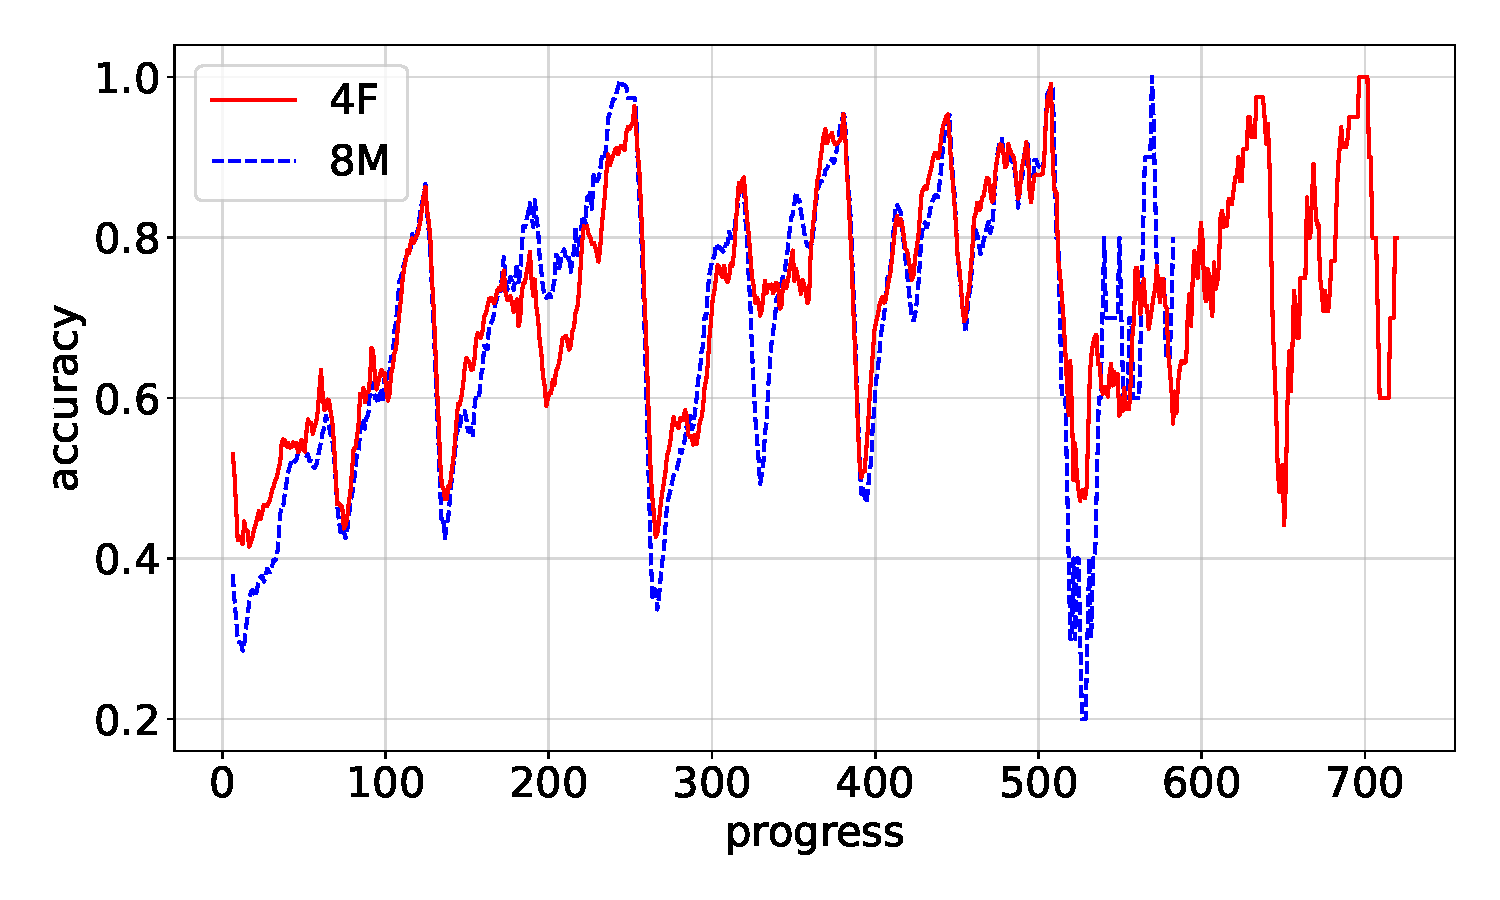
\includegraphics[width=\linewidth]{pdf/compare/EXP6_NT4F_and_NT8M/accuracy.pdf}
    \caption{正確度}
    \label{fig:EXP6_:NT4F_and_NT8M_accuracy}
\end{subfigure}
\begin{subfigure}[b]{0.49\linewidth}
    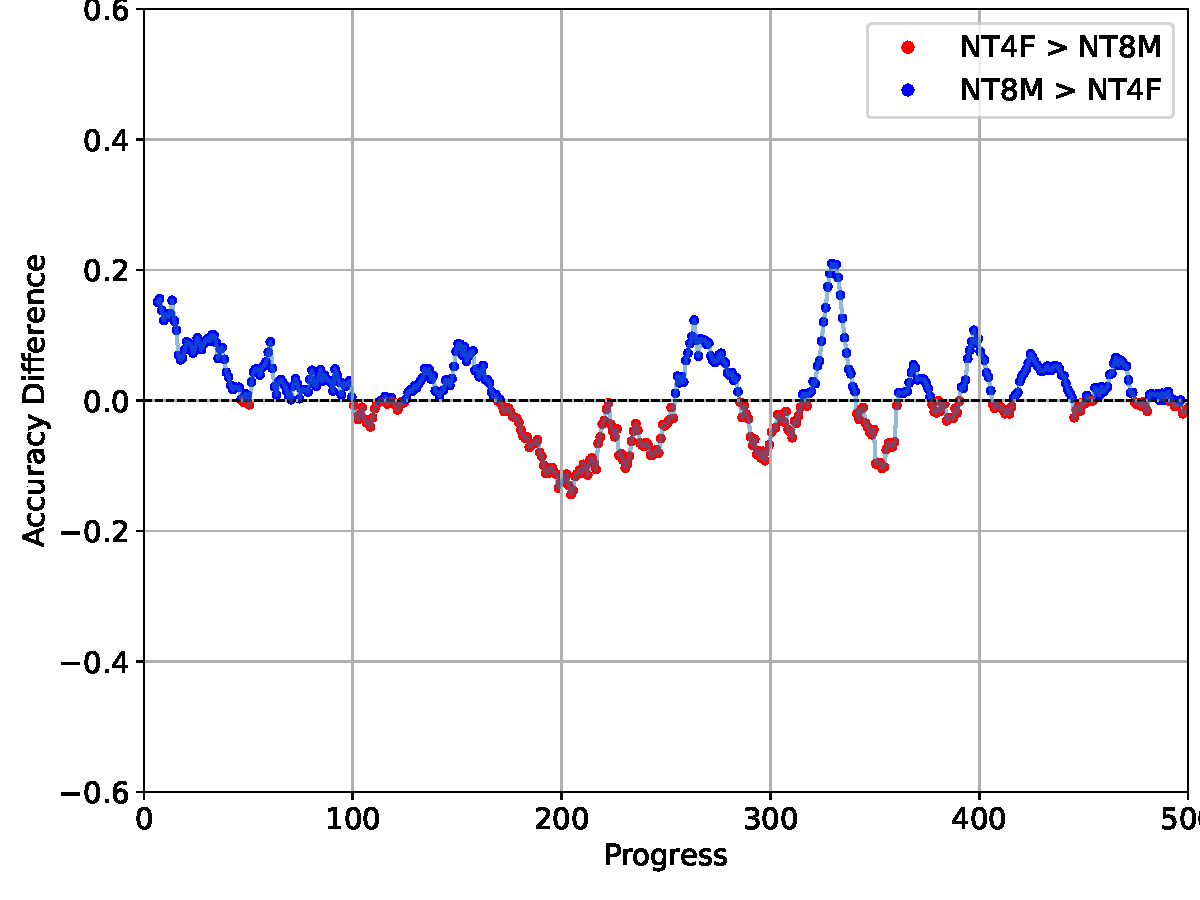
\includegraphics[width=\linewidth]{pdf/compare/EXP6_NT4F_and_NT8M/acc_diff_plot.pdf}
    \caption{正確度の差分}
    \label{fig:EXP6_NT4F_and_NT8M_acc_diff}
\end{subfigure}
\begin{subfigure}[b]{0.49\linewidth}
    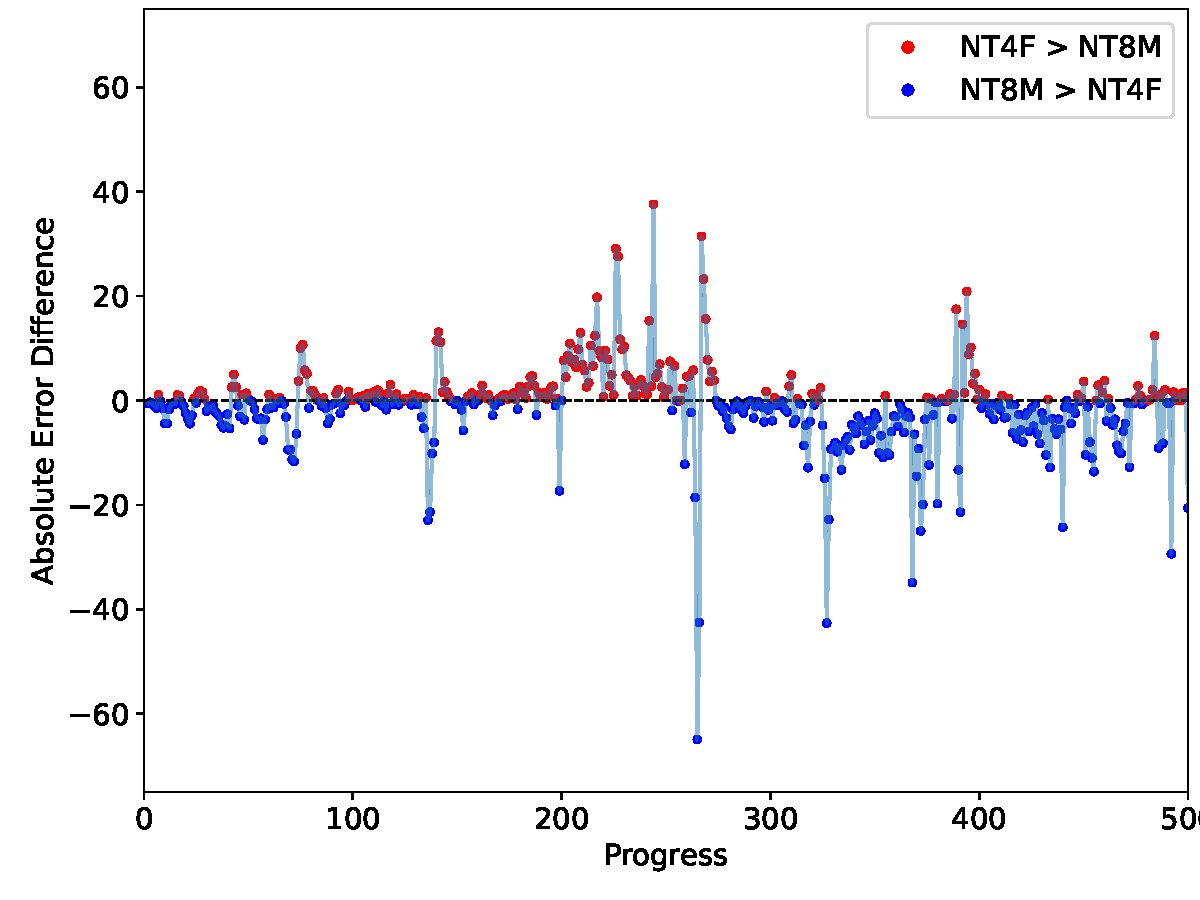
\includegraphics[width=\linewidth]{pdf/compare/EXP6_NT4F_and_NT8M/error_abs_diff_plot.pdf}
    \caption{絶対誤差の差分}
    \label{fig:EXP6_NT4F_and_NT8M_error_abs_diff}
\end{subfigure}
\begin{subfigure}[b]{0.49\linewidth}
    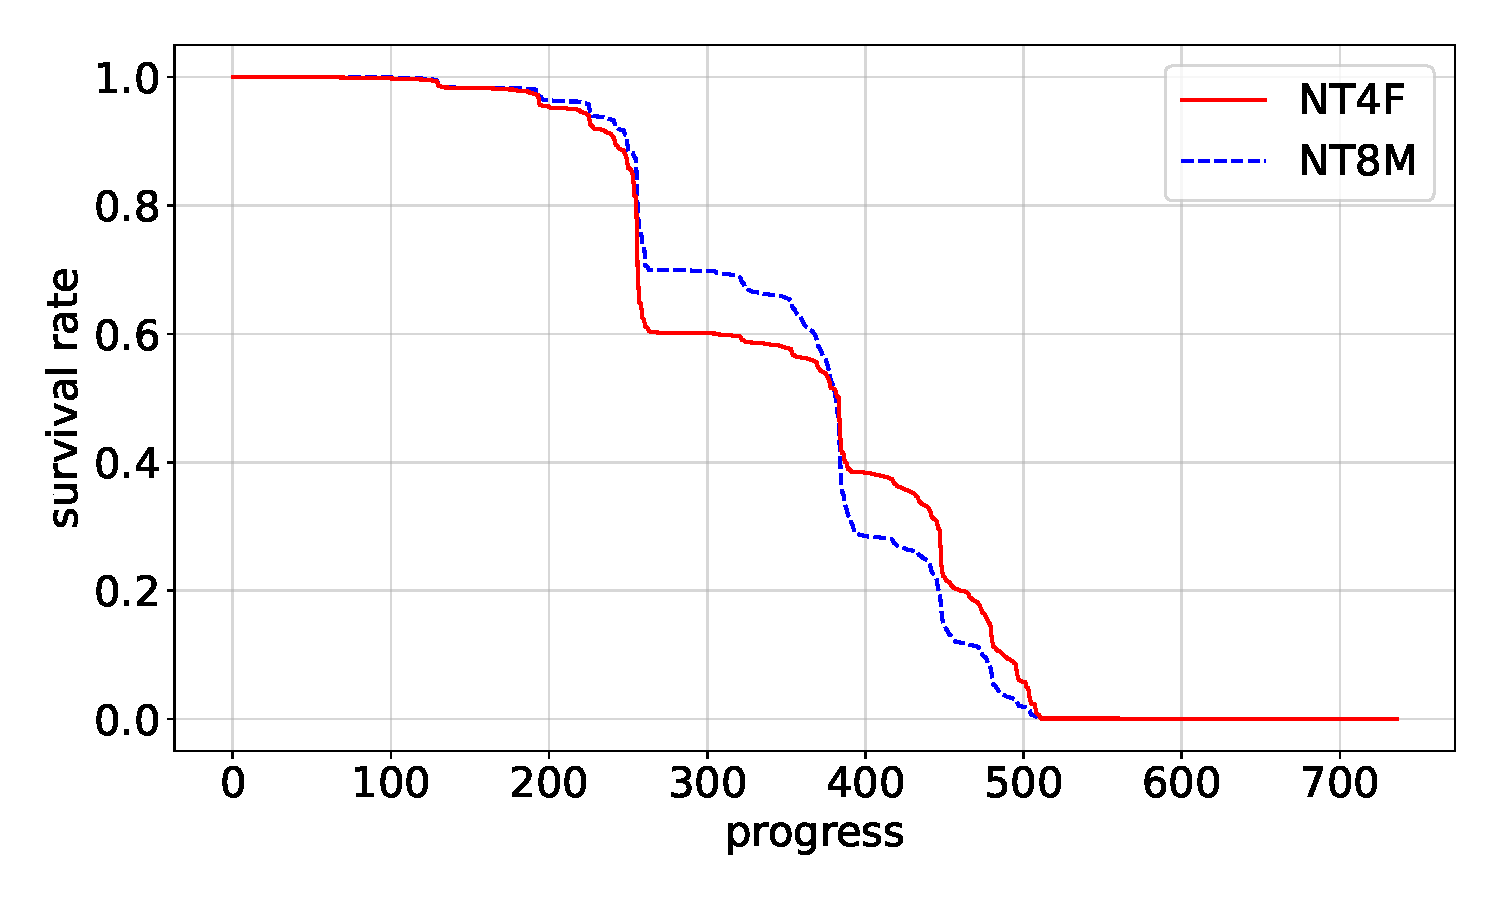
\includegraphics[width=\linewidth]{pdf/compare/EXP6_NT4F_and_NT8M/survival.pdf}
    \caption{生存率}
    \label{figEXP6_:NT4F_and_NT8M_survival}
\end{subfigure}
\caption{NT4FとNT8Mの比較結果(深さ6)}
\label{fig:EXP6_NT4FとNT8M_results}
\end{figure}
    

\begin{figure}[t]
\centering
\begin{subfigure}[b]{0.49\linewidth}
    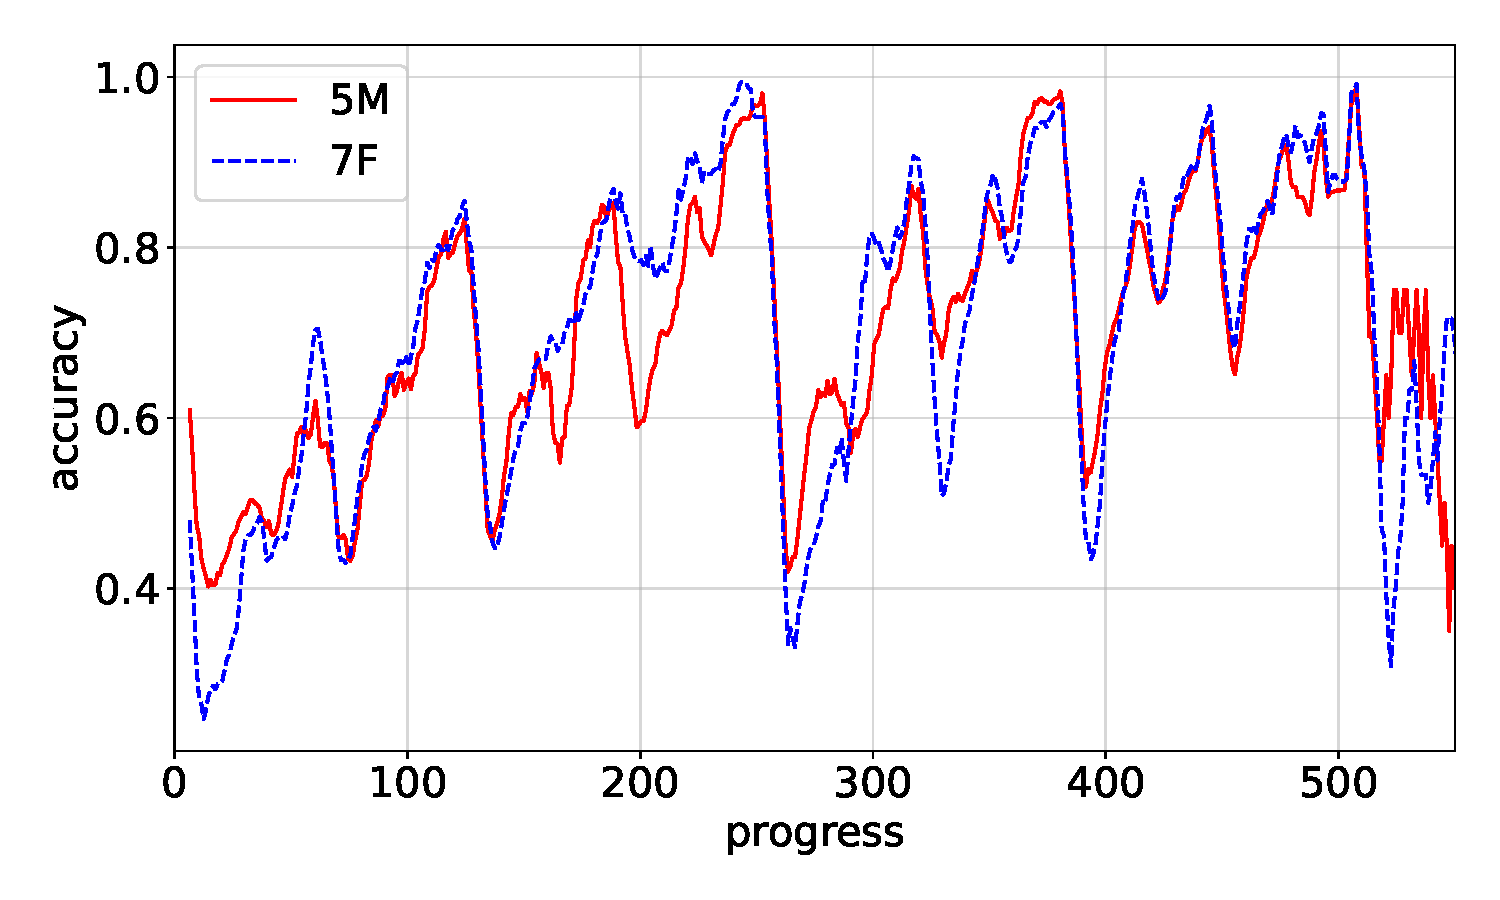
\includegraphics[width=\linewidth]{pdf/compare/EXP6_NT5M_and_NT7F/accuracy.pdf}
    \caption{正確度}
    \label{fig:EXP6_NT5M_and_NT7F_accuracy}
\end{subfigure}
\begin{subfigure}[b]{0.49\linewidth}
    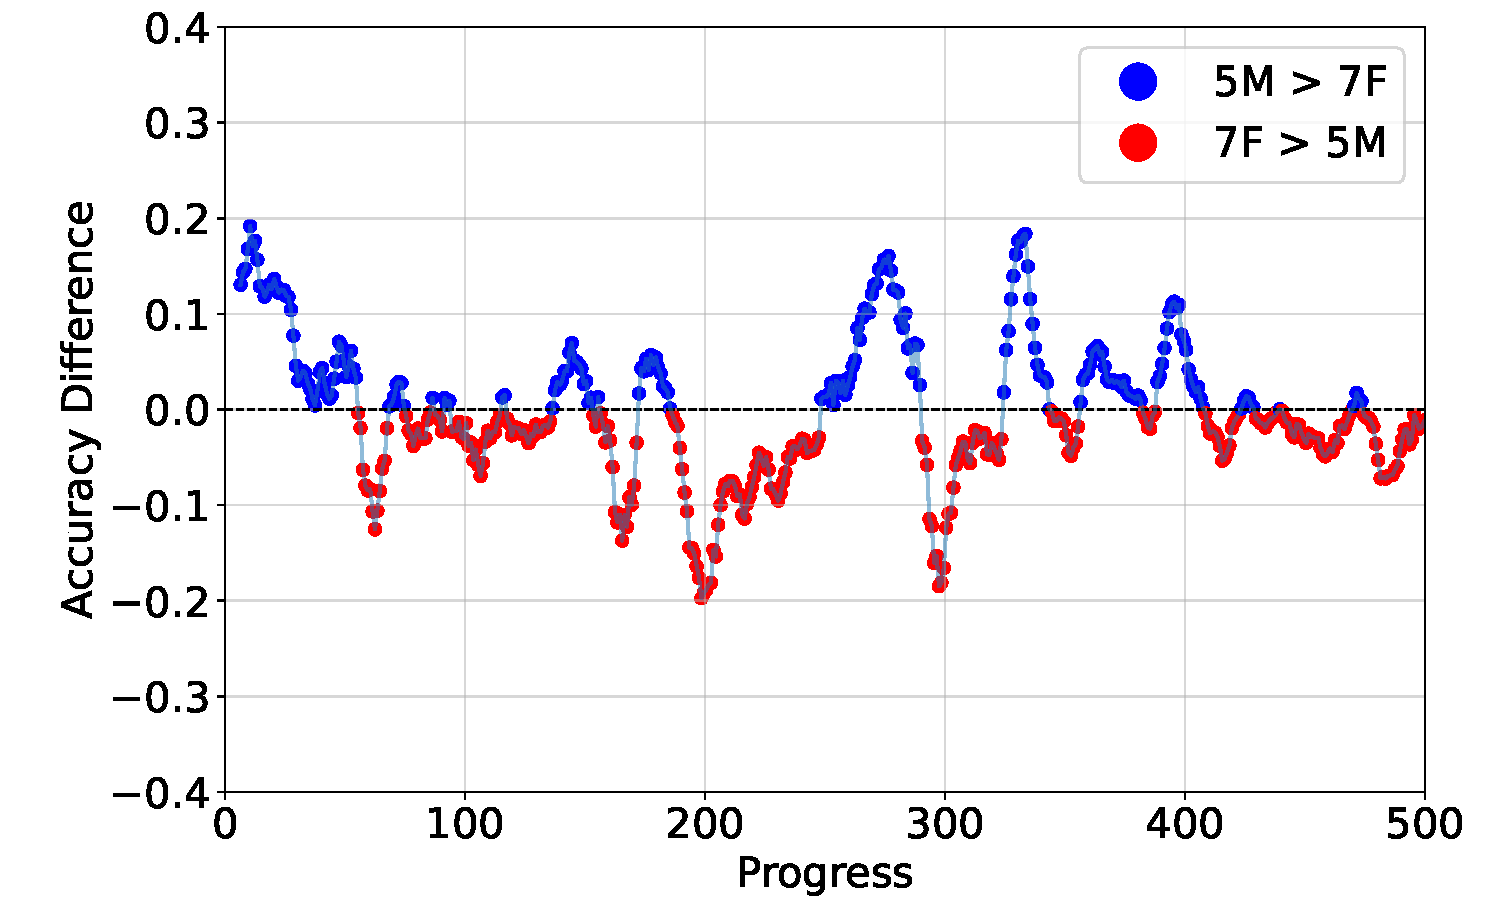
\includegraphics[width=\linewidth]{pdf/compare/EXP6_NT5M_and_NT7F/acc_diff_plot.pdf}
    \caption{正確度の差分}
    \label{fig:EXP6_NT5M_and_NT7F_acc_diff}
\end{subfigure}
\begin{subfigure}[b]{0.49\linewidth}
    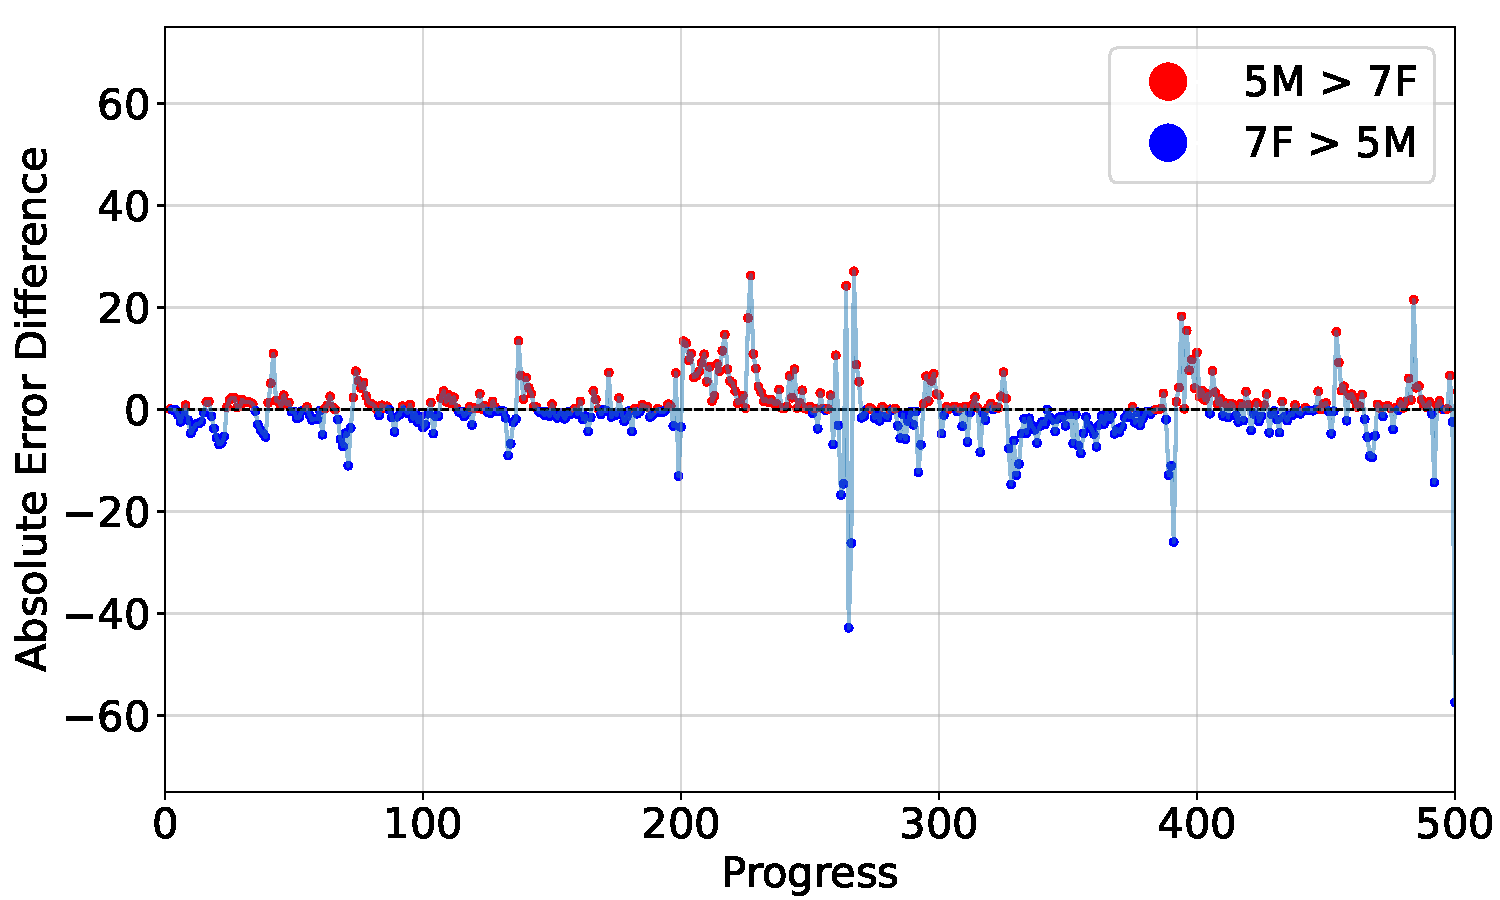
\includegraphics[width=\linewidth]{pdf/compare/EXP6_NT5M_and_NT7F/error_abs_diff_plot.pdf}
    \caption{絶対誤差の差分}
    \label{fig:EXP6_NT5M_and_NT7F_error_abs_diff}
\end{subfigure}
\begin{subfigure}[b]{0.49\linewidth}
    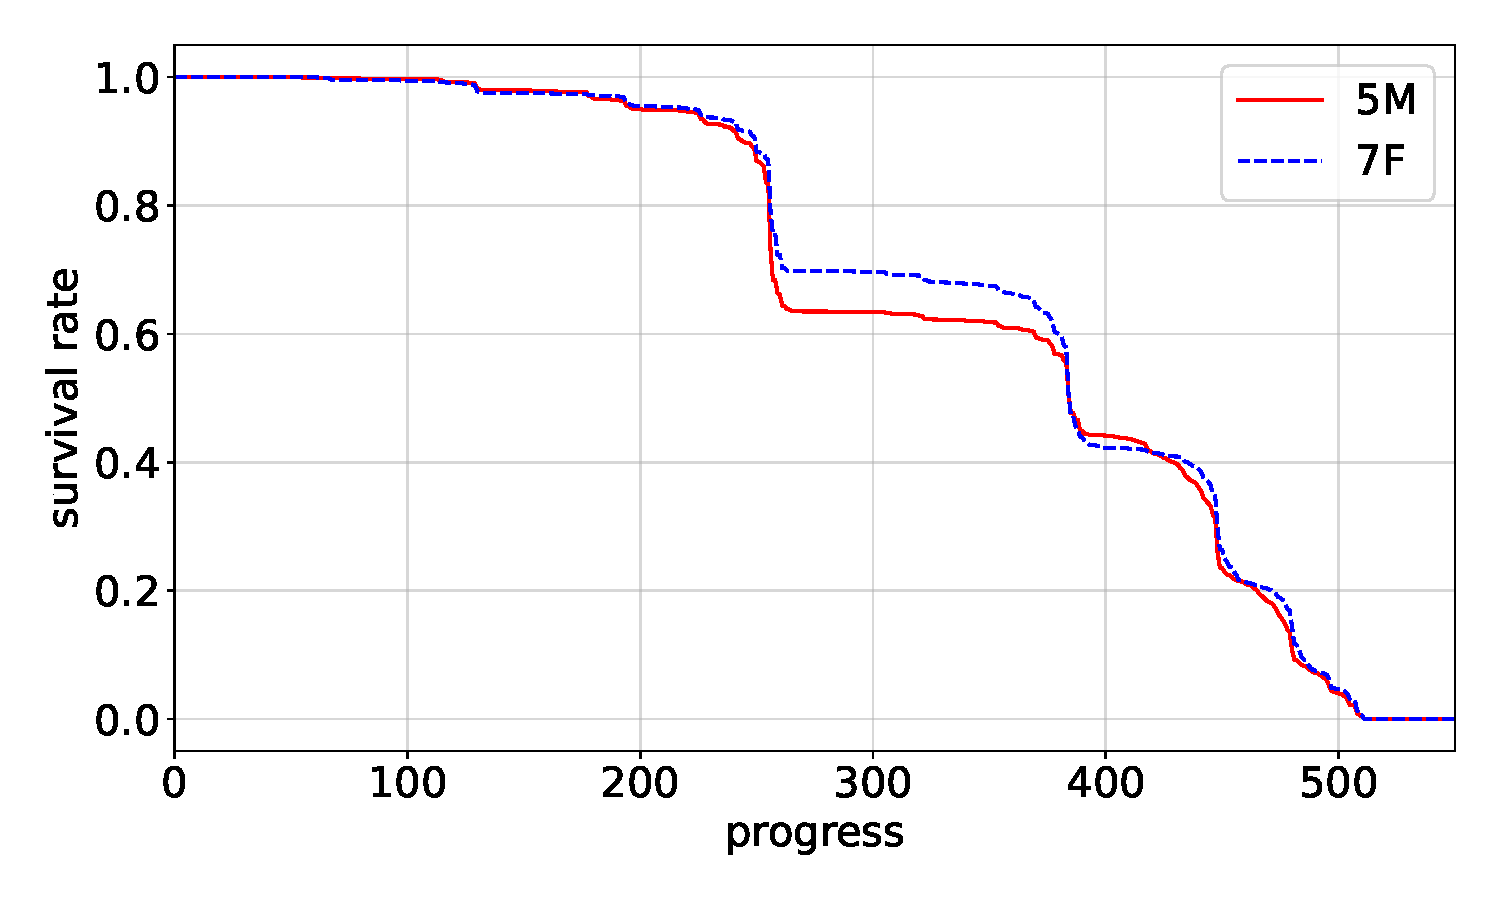
\includegraphics[width=\linewidth]{pdf/compare/EXP6_NT5M_and_NT7F/survival.pdf}
    \caption{生存率}
    \label{fig:EXP6_NT5M_and_NT7F_survival}
\end{subfigure}
\caption{NT5MとNT7Fの比較結果(深さ6)}
\label{fig:EXP6_NT5M_and_NT7F_results}
\end{figure}

図\ref{fig:EXP6_NT4FとNT8M_results}と図\ref{fig:EXP6_NT5M_and_NT7F_results}は、
図\ref{fig:NT4FとNT8M_results}と図\ref{fig:NT5M_and_NT7F_results}のExpectimax探索深さ6を組み合わせたプレイヤである。
図\ref{fig:EXP6_:NT4F_and_NT8M_accuracy}と図\ref{fig:EXP6_NT4F_and_NT8M_acc_diff}を見ると正確性はNT4Fの方が良い
図\ref{fig:EXP_6_NT5M_and_NT7F_accuracy}と図\ref{fig:EXP_6_NT5M_and_NT7F_acc_diff}を見ると正確性はNT5Mの方が良い
図\ref{fig:EXP6_NT4F_and_NT8M_error_abs_diff}と図\ref{fig:EXP6_NT5M_and_NT7F_error_abs_diff}は絶対誤差の差分を示していて、
ここは探索を加えたことで上下の振れ幅がとても小さくなっていることが分かるが結局どちらの結果からも特徴的な形は見られなかった。
